\chapter{Multilateriacja}\label{chap:multilateration}

\section{Przygotowanie danych wejściowych}

Aby otrzymać poprawne wyniki algorytmu multilateracji, dane wejściowe, w naszym przypadku odległości między węzłami odbiorczymi a nadajnikiem, powinny być jak najbliższe rzeczywistym odległościom z możliwie małymi odchyleniami. Będziemy kontynuować usprawnianie metod uzyskiwania poprawnych wyników zapoczątkowane w rozdziale poprzednim.

\subsection{Korekcja odległości}

W wynikach eksperymentów porównawczych metod synchronizacji czasu węzłów przeprowadzonych w rozdziale~\ref{chap:time_sync}.\ zaobserwowaliśmy skalowanie wyników na pierwszy rzut oka zachowujące się liniowo. Przyjrzyjmy się teraz dokładnie temu zjawisku. W tym i kolejnych przypadkach będziemy używać już jedynie synchronizacji sprzętowej z użyciem mikrofonów, ze względu na brak konieczności dodatkowej kalibracji przesunięcia punktu 0.

Prawdopodobnym powodem skalowania obliczanych odległości mogą być różnice w rejestracji sygnału mikrofonowego odczytywanego przez mikrokontroler. Poniższe wykresy są wynikiem czterech kolejnych eksperymentów, w których jedyną zmienną była czułość zintegrowanego wzmacniacza mikrofonu. Wzmacniacz ten nie pozwala na precyzyjną regulację, a jedynie na zmianę rezystancji wbudowanego potencjometru. Ponieważ przedział czułości odpowiadający wykrywaniu sygnału węzła nadającego przy jednoczesnym zminimalizowaniu fałszywych aktywacji jest niewielki (około $\frac{1}{8}$ obrotu potencjometru), cztery zbadane przypadki nie dzielą równo badanego zakresu. Rozpoczynając od największej możliwej czułości, przy każdym kolejnym eksperymencie zmniejszano ją, póki pozwalała wciąż na wykrywanie sygnału z badanych odległości.

\begin{figure}[H]
    \centering
    \begin{subfigure}{\textwidth}
        \centering
        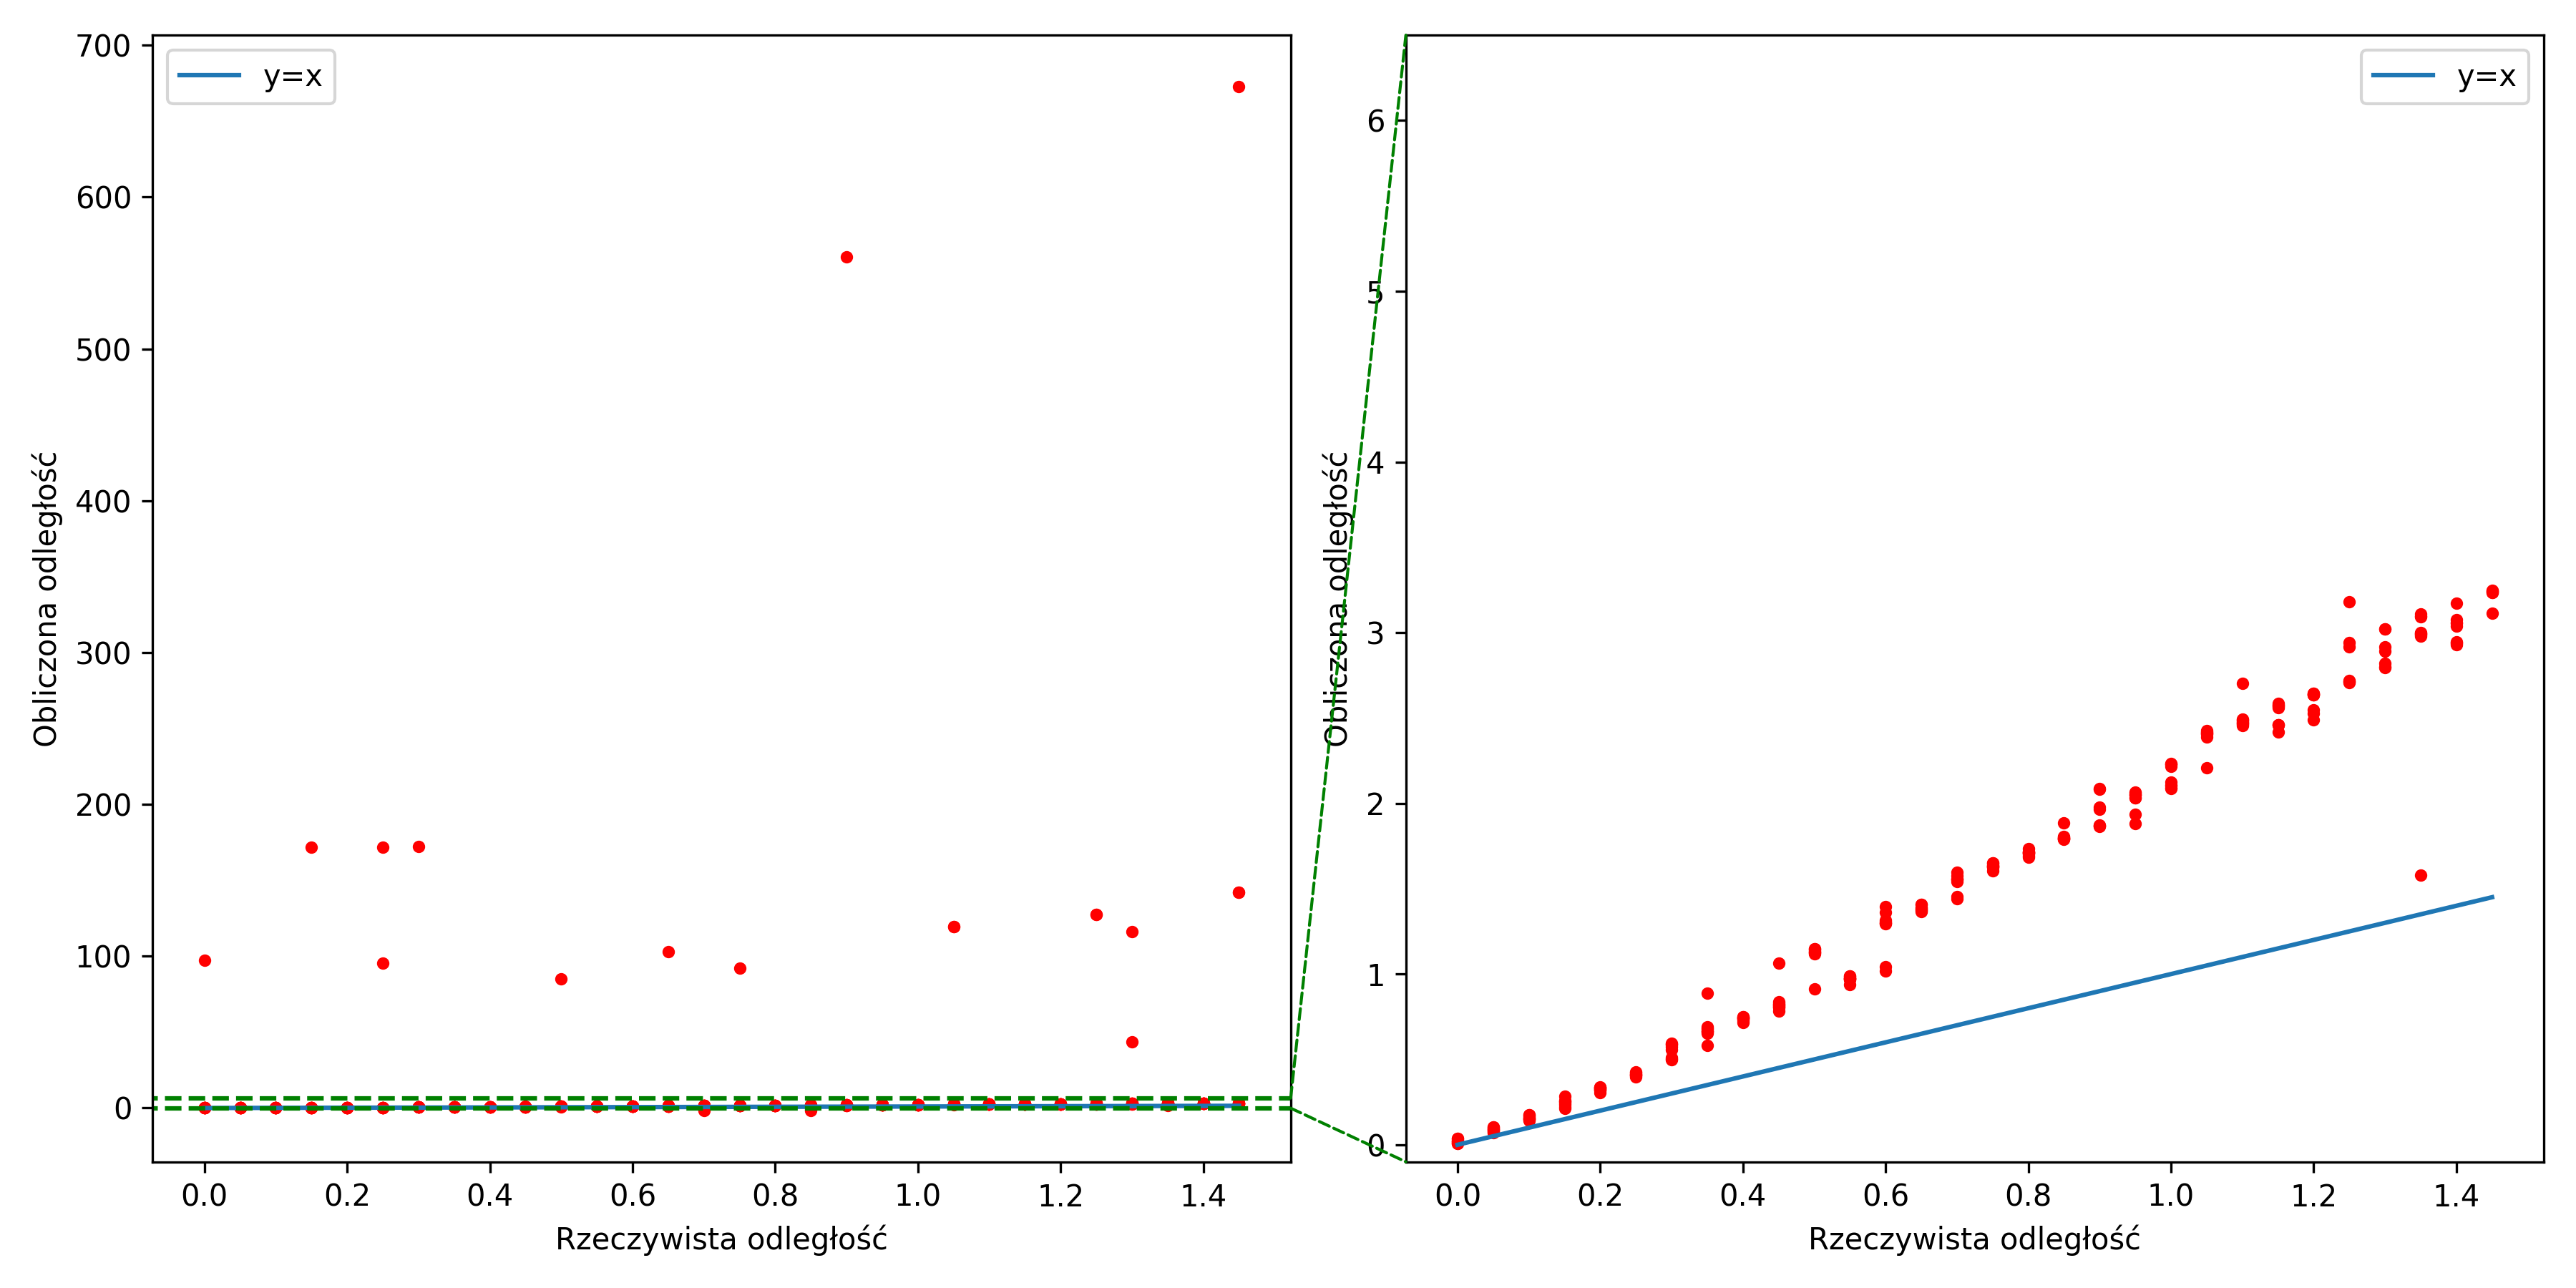
\includegraphics[width=\textwidth]{pics/mic_sync_dist/dists_long_0.png}
        \caption{pomiar 1.}
        \label{pic:slope_test_0}
    \end{subfigure}
\end{figure}
\begin{figure}[H]
    \ContinuedFloat\centering
    \begin{subfigure}{\textwidth}
        \centering
        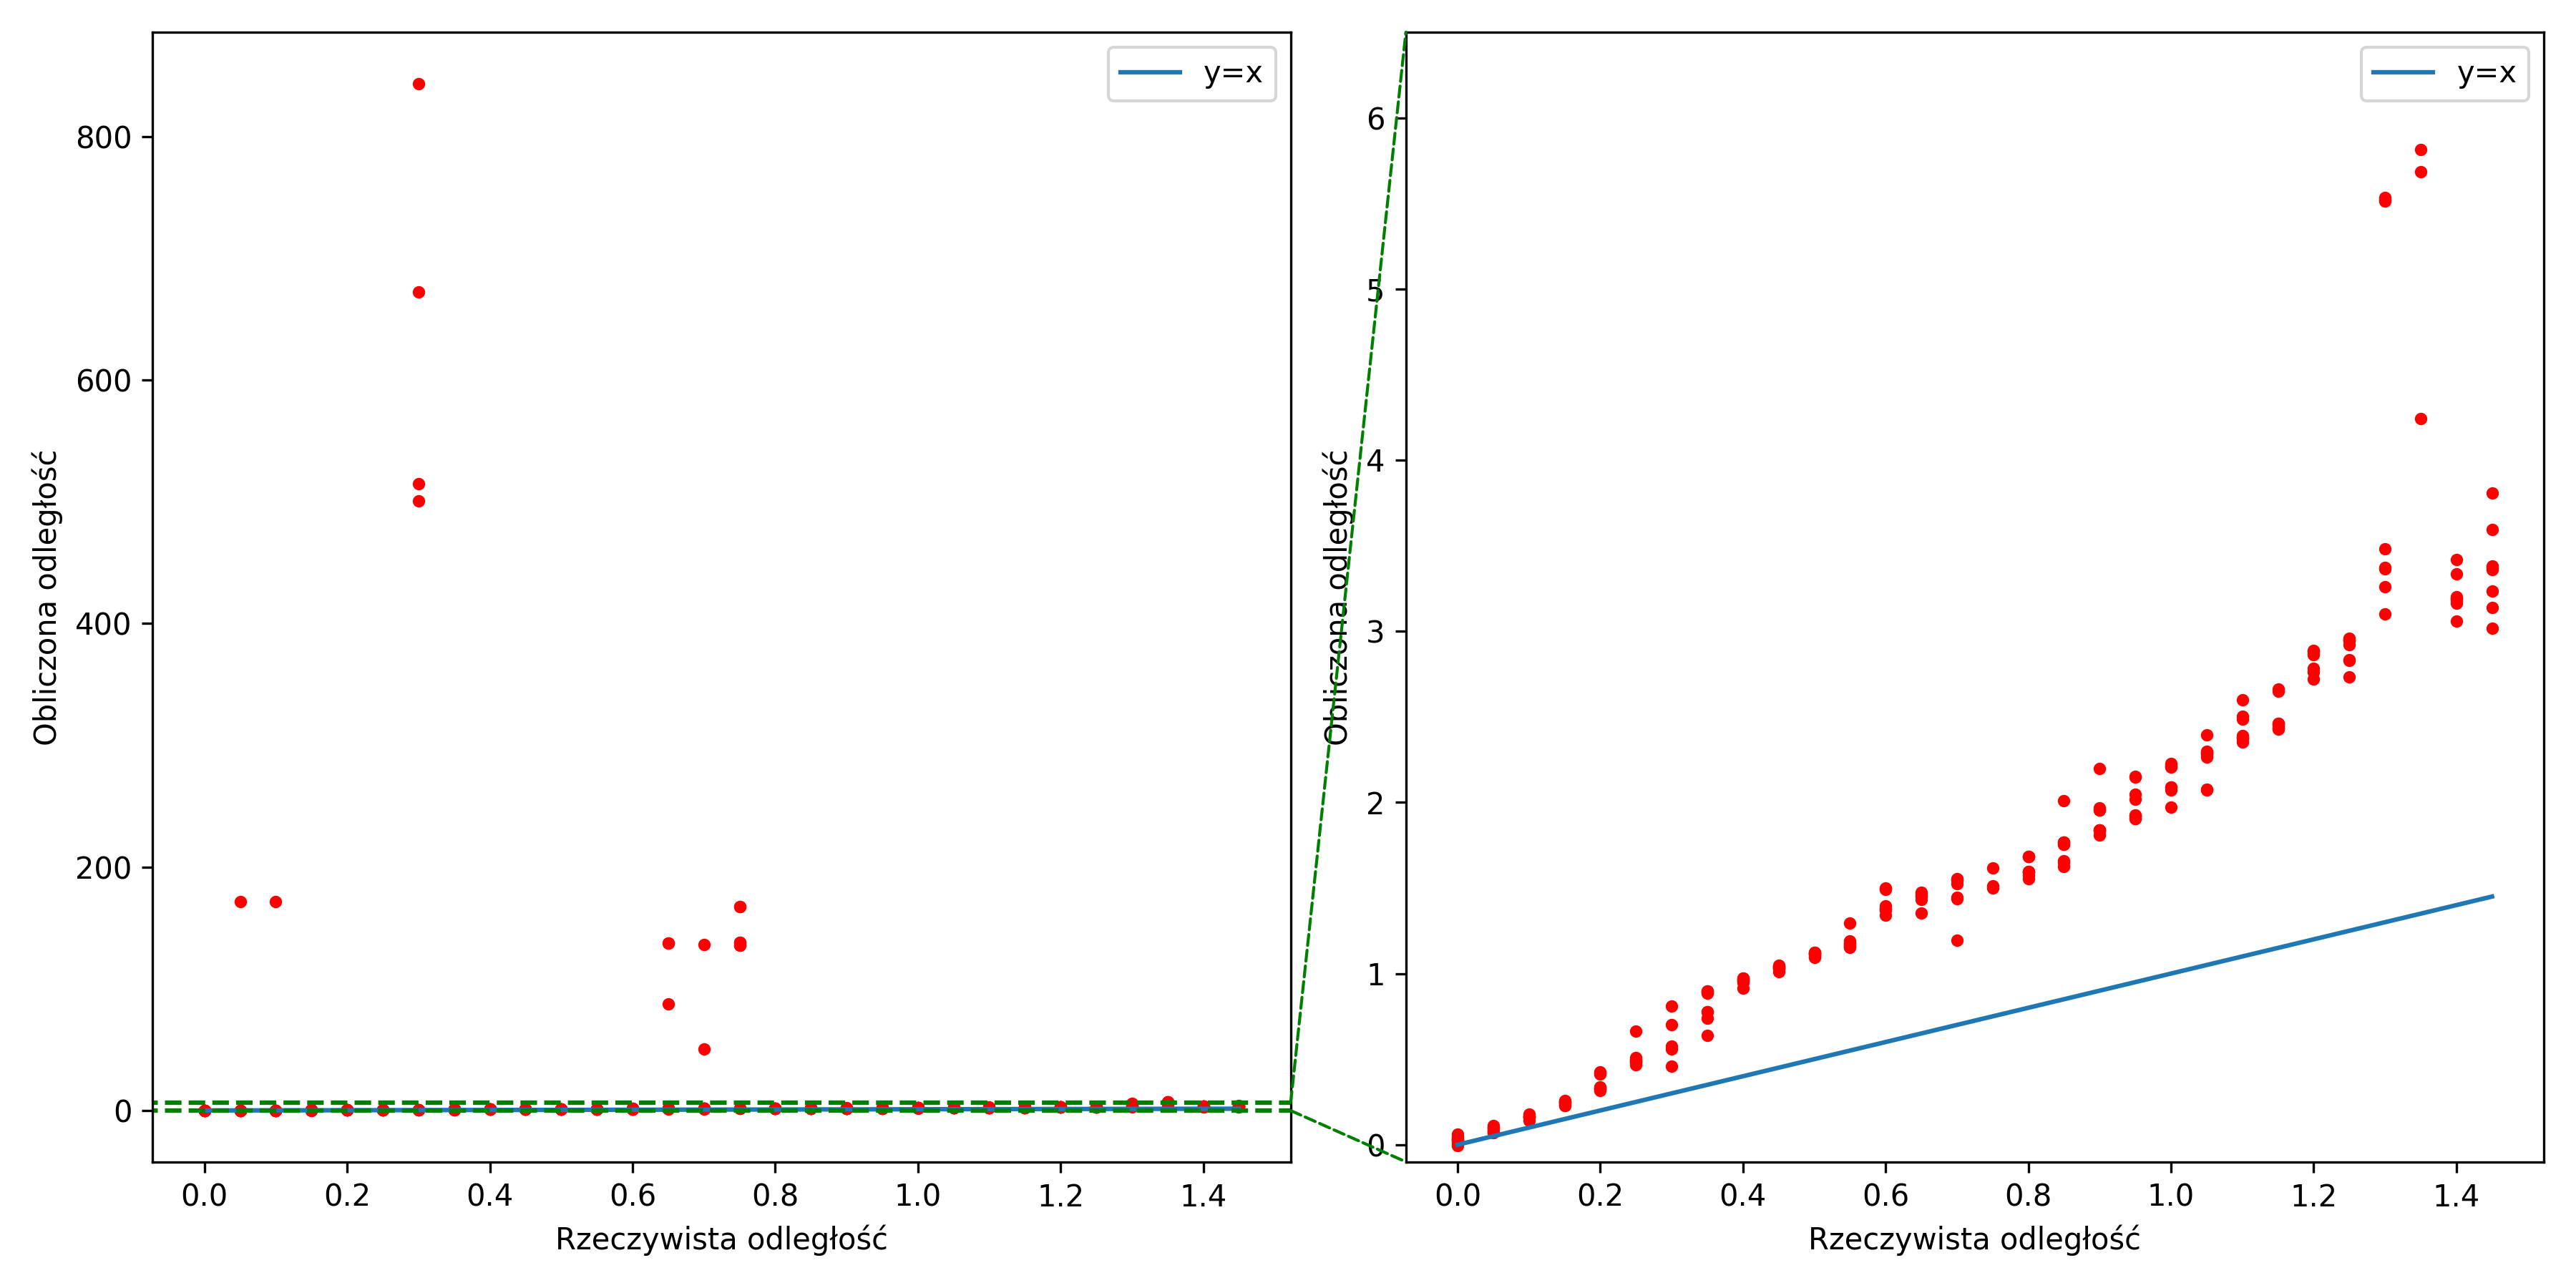
\includegraphics[width=\textwidth]{pics/mic_sync_dist/dists_long_1.png}
        \caption{pomiar 2.}
        \label{pic:slope_test_1}
    \end{subfigure}
\end{figure}
\begin{figure}[H]
    \ContinuedFloat\centering
    \begin{subfigure}{\textwidth}
        \centering
        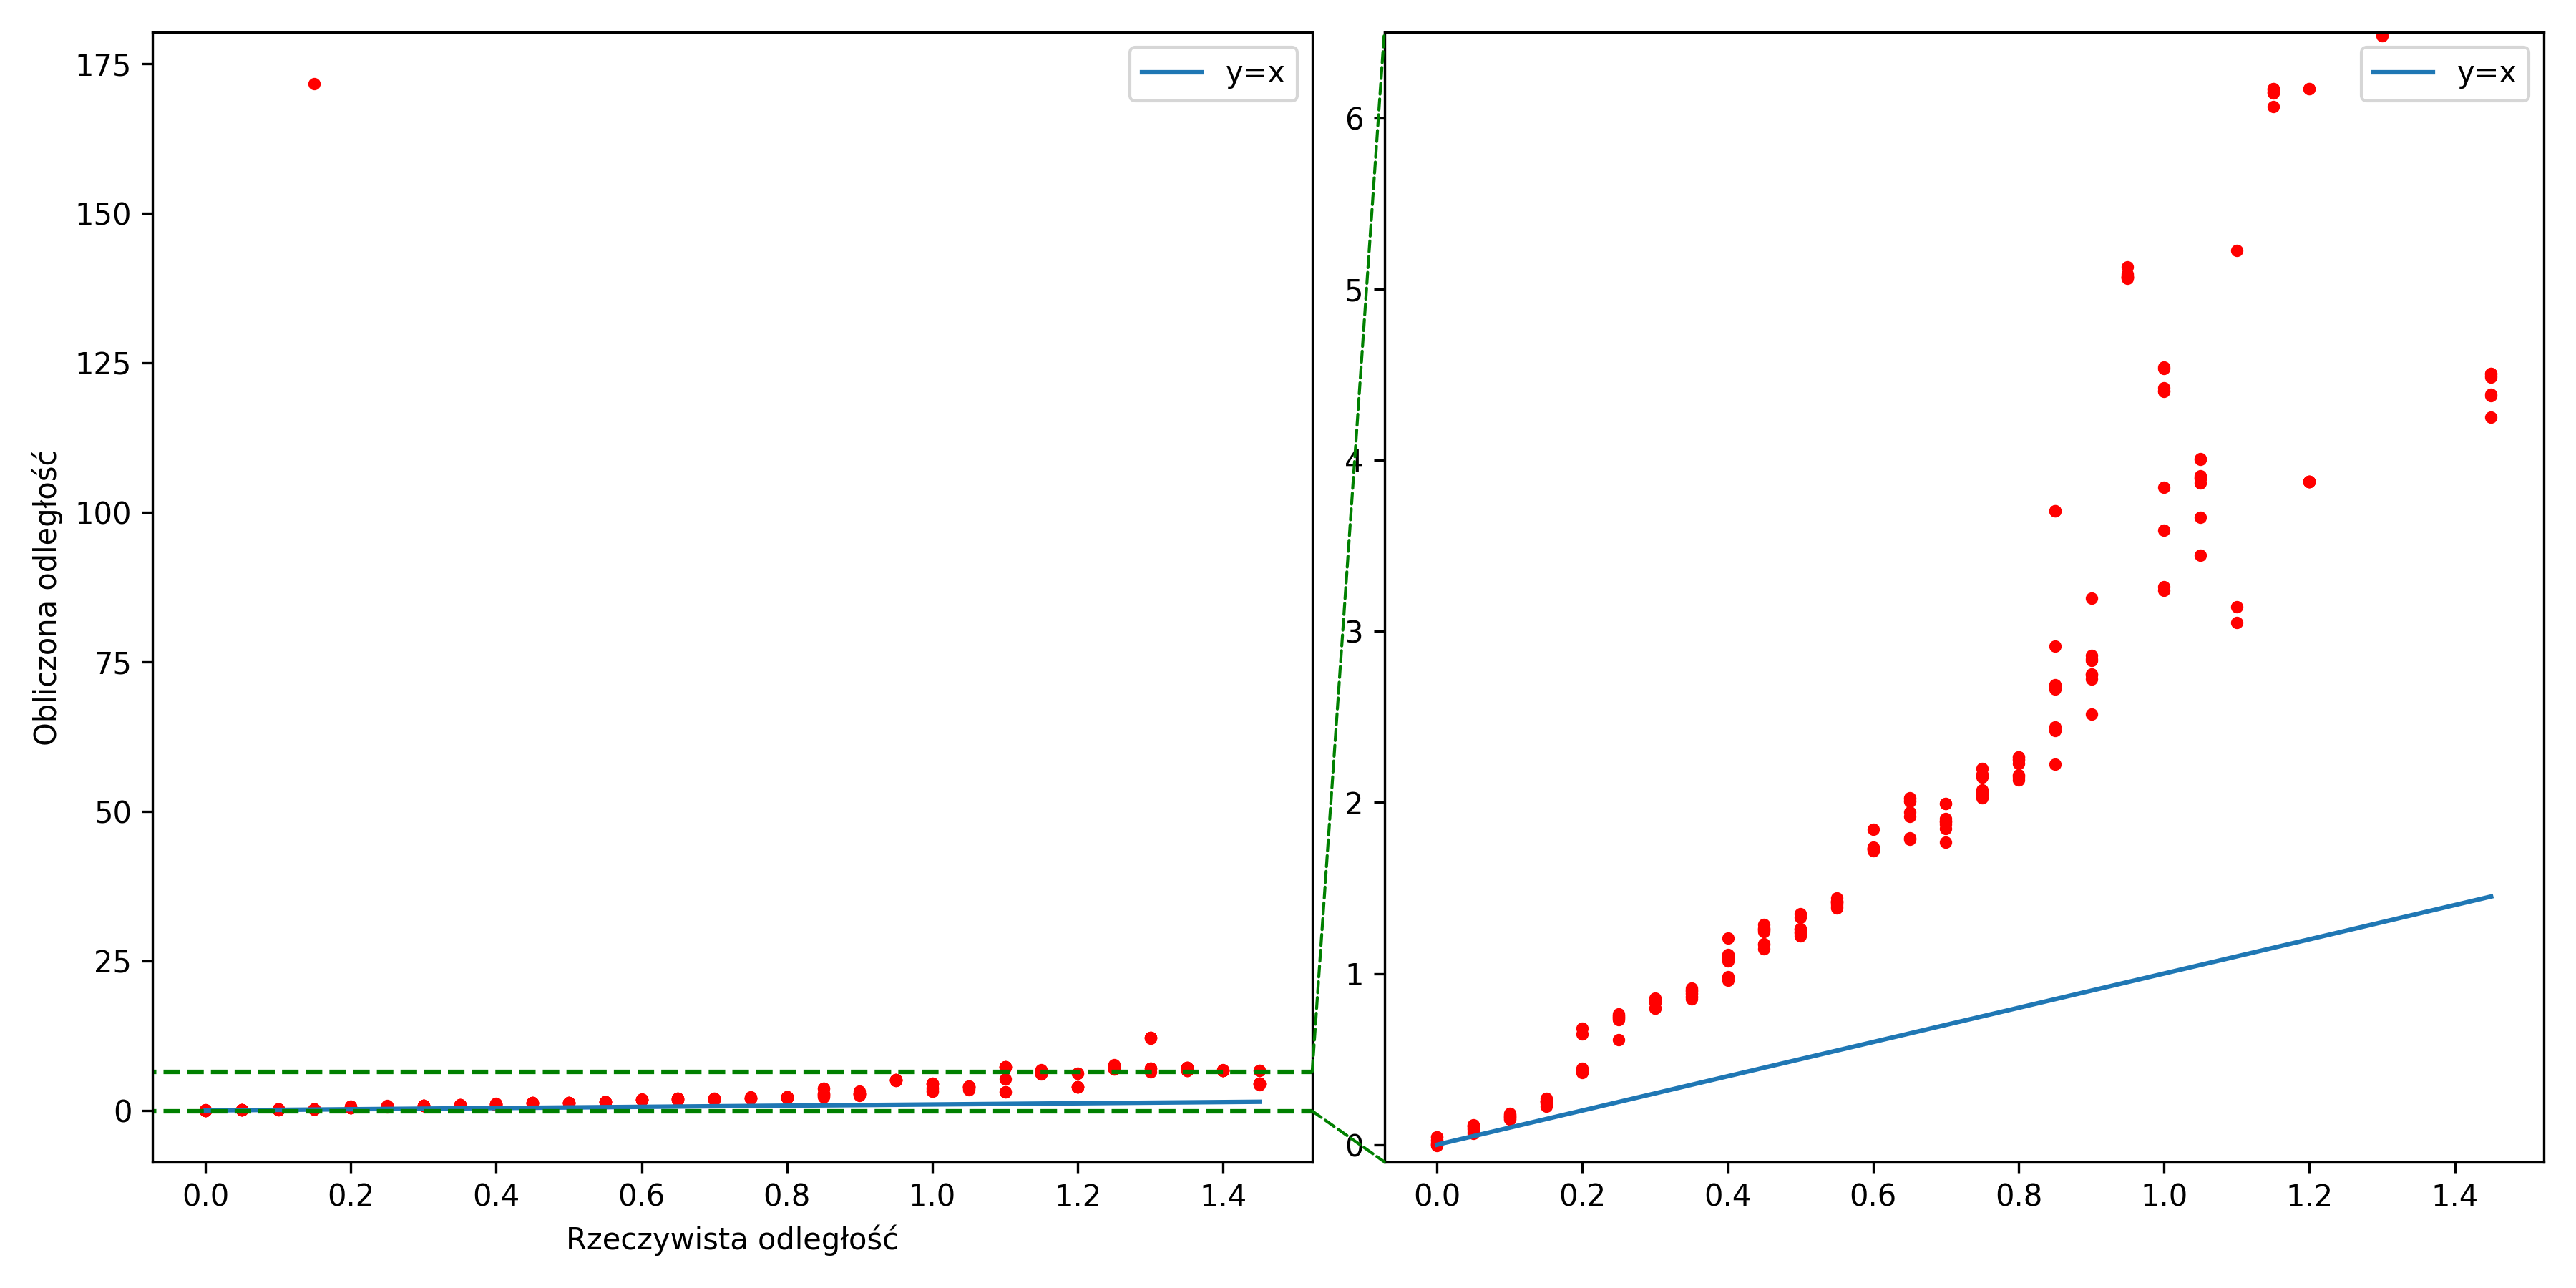
\includegraphics[width=\textwidth]{pics/mic_sync_dist/dists_long_2.png}
        \caption{pomiar 3.}
        \label{pic:slope_test_2}
    \end{subfigure}
\end{figure}
\begin{figure}[H]
    \ContinuedFloat\centering
    \begin{subfigure}{\textwidth}
        \centering
        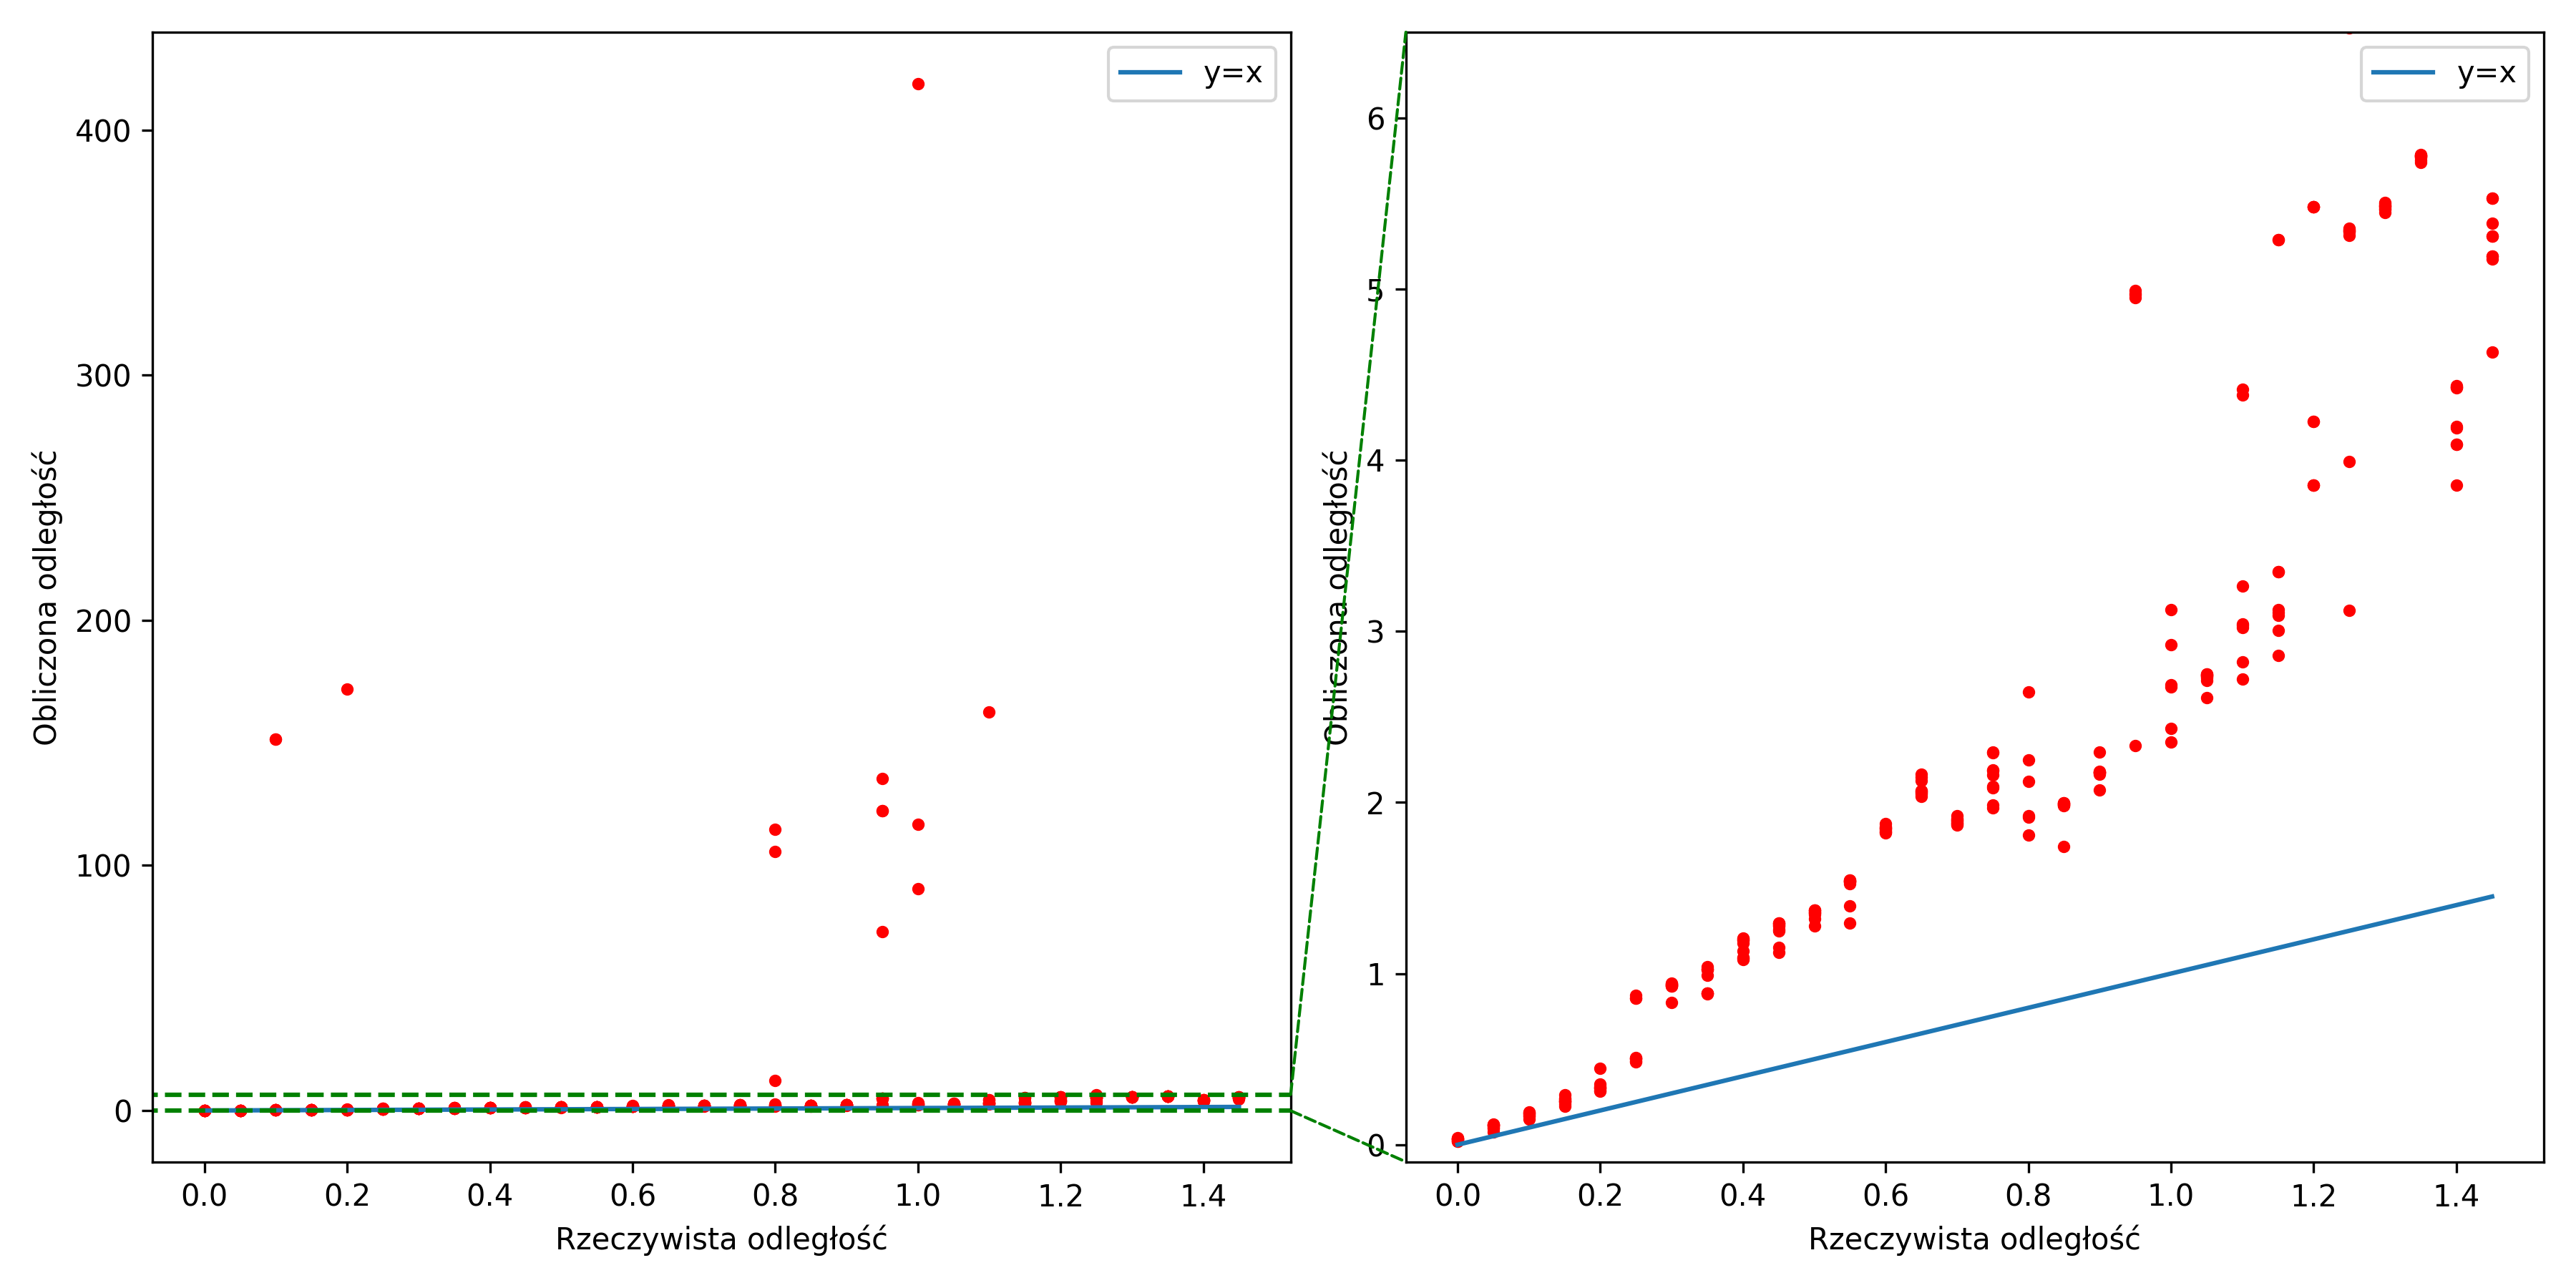
\includegraphics[width=\textwidth]{pics/mic_sync_dist/dists_long_3.png}
        \caption{pomiar 4.}
        \label{pic:slope_test_3}
    \end{subfigure}
    \caption[Pomiar obliczanych odległości]{Pomiar obliczanych odległości. Diagram po prawej stanowi powiększenie zaznaczonego obszaru diagramu po lewej.}
    \label{fig:slope_test}
\end{figure}

Aby lepiej odczytać informacje z wykresu uśrednijmy pomiary dla każdej z badanych odległości i dodajmy do nich funkcje liniowe o współczynniku otrzymanym przy pomocy regresji liniowej z tychże uśrednionych punktów.

\begin{figure}[H]
    \centering
    \begin{subfigure}{0.5\textwidth}
        \centering
        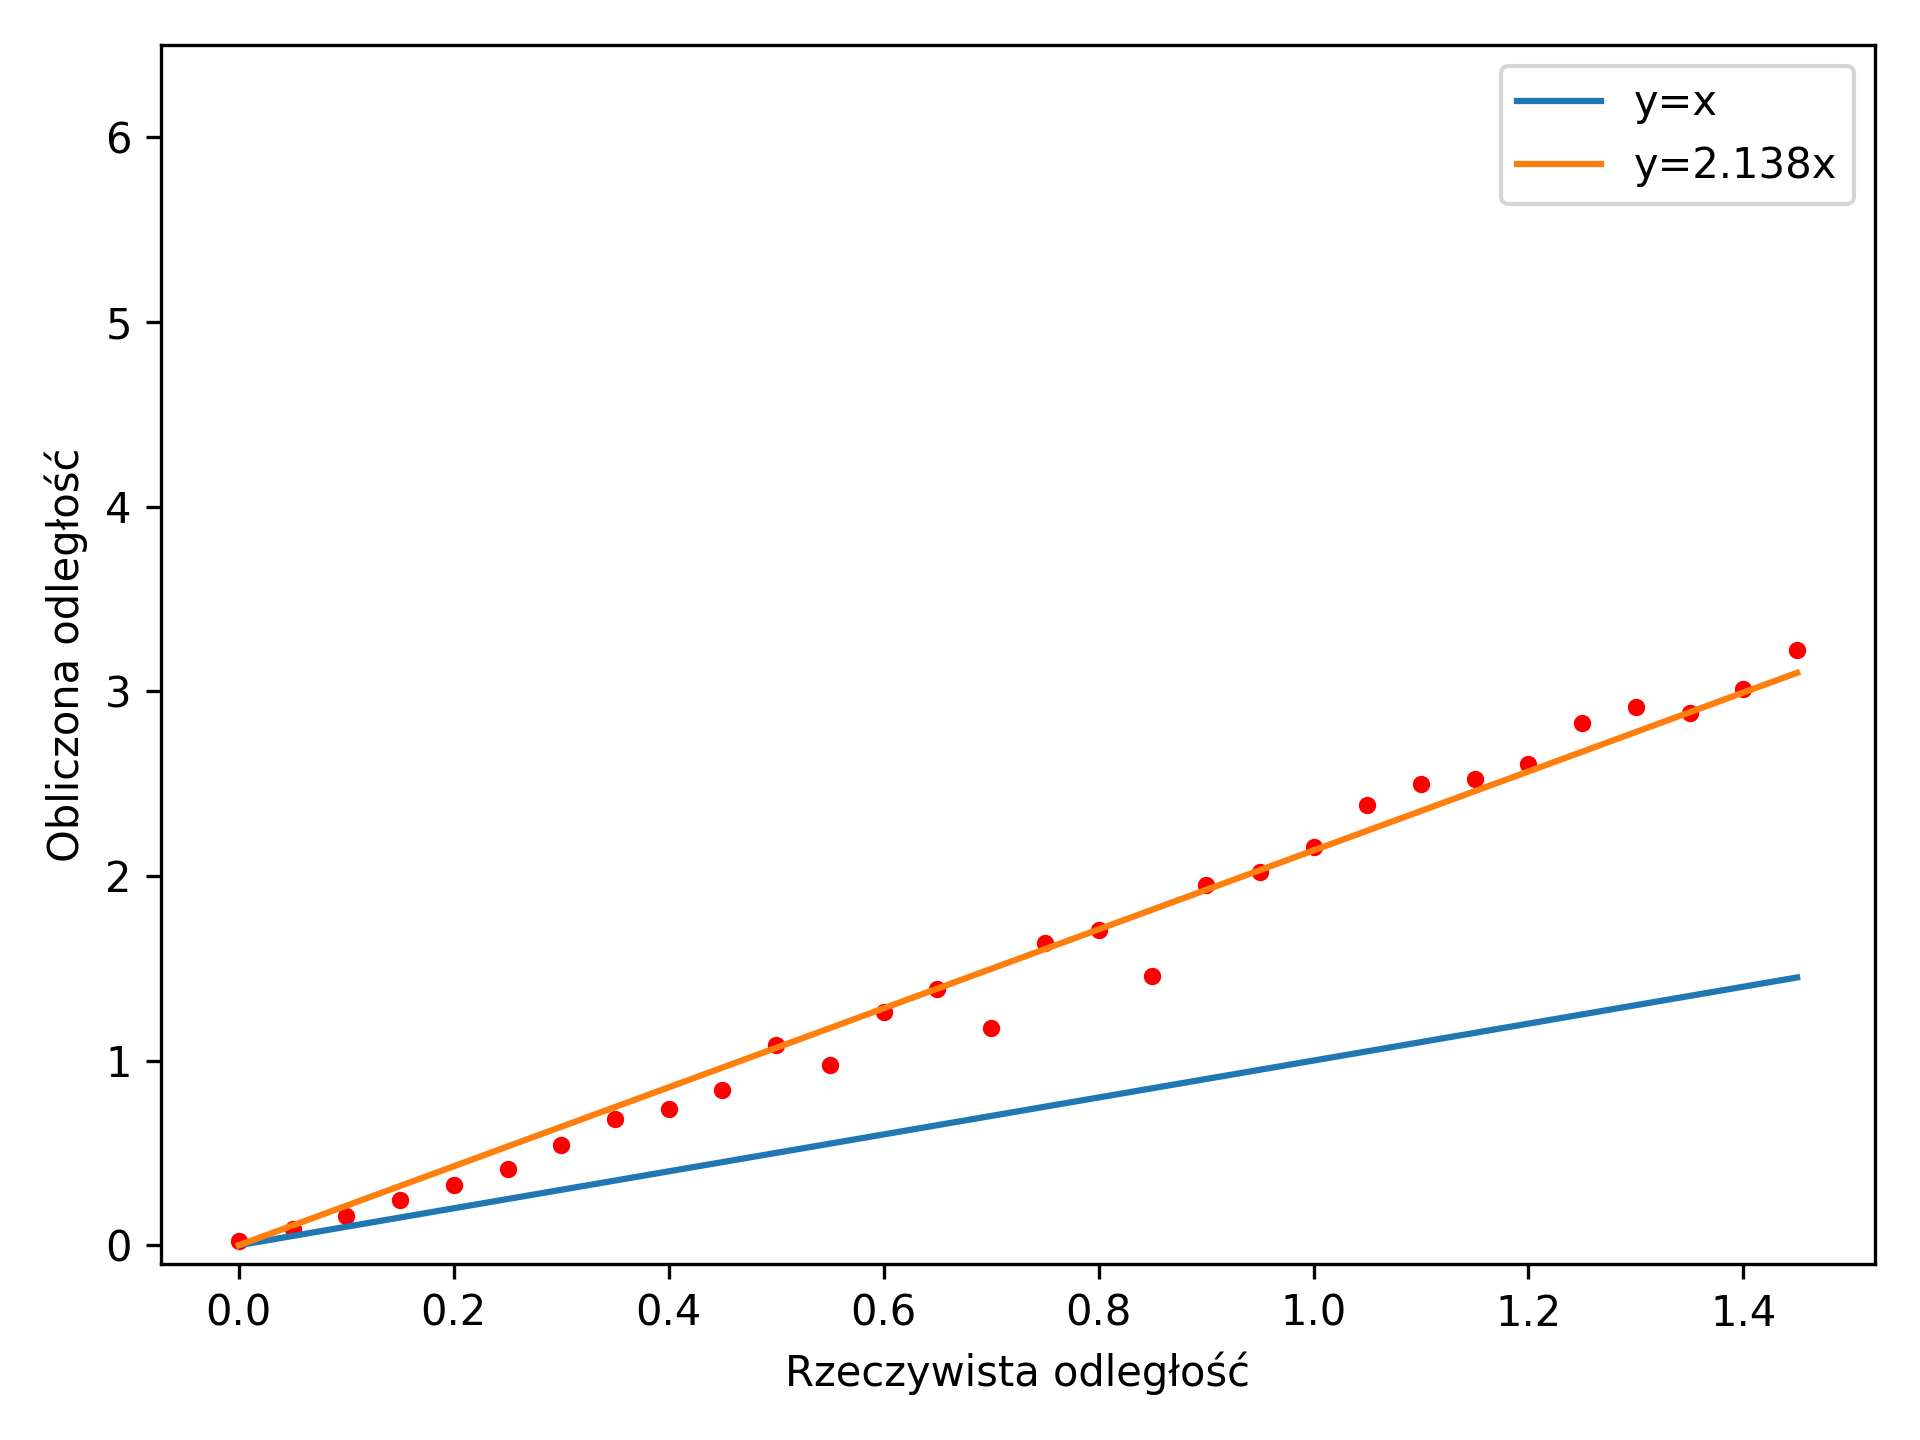
\includegraphics[width=\textwidth]{pics/mic_sync_dist/dists_close_long_0_mean.png}
        \caption{pomiar 1.}
        \label{pic:slope_test_mean_0}
    \end{subfigure}%
    \begin{subfigure}{0.5\textwidth}
        \centering
        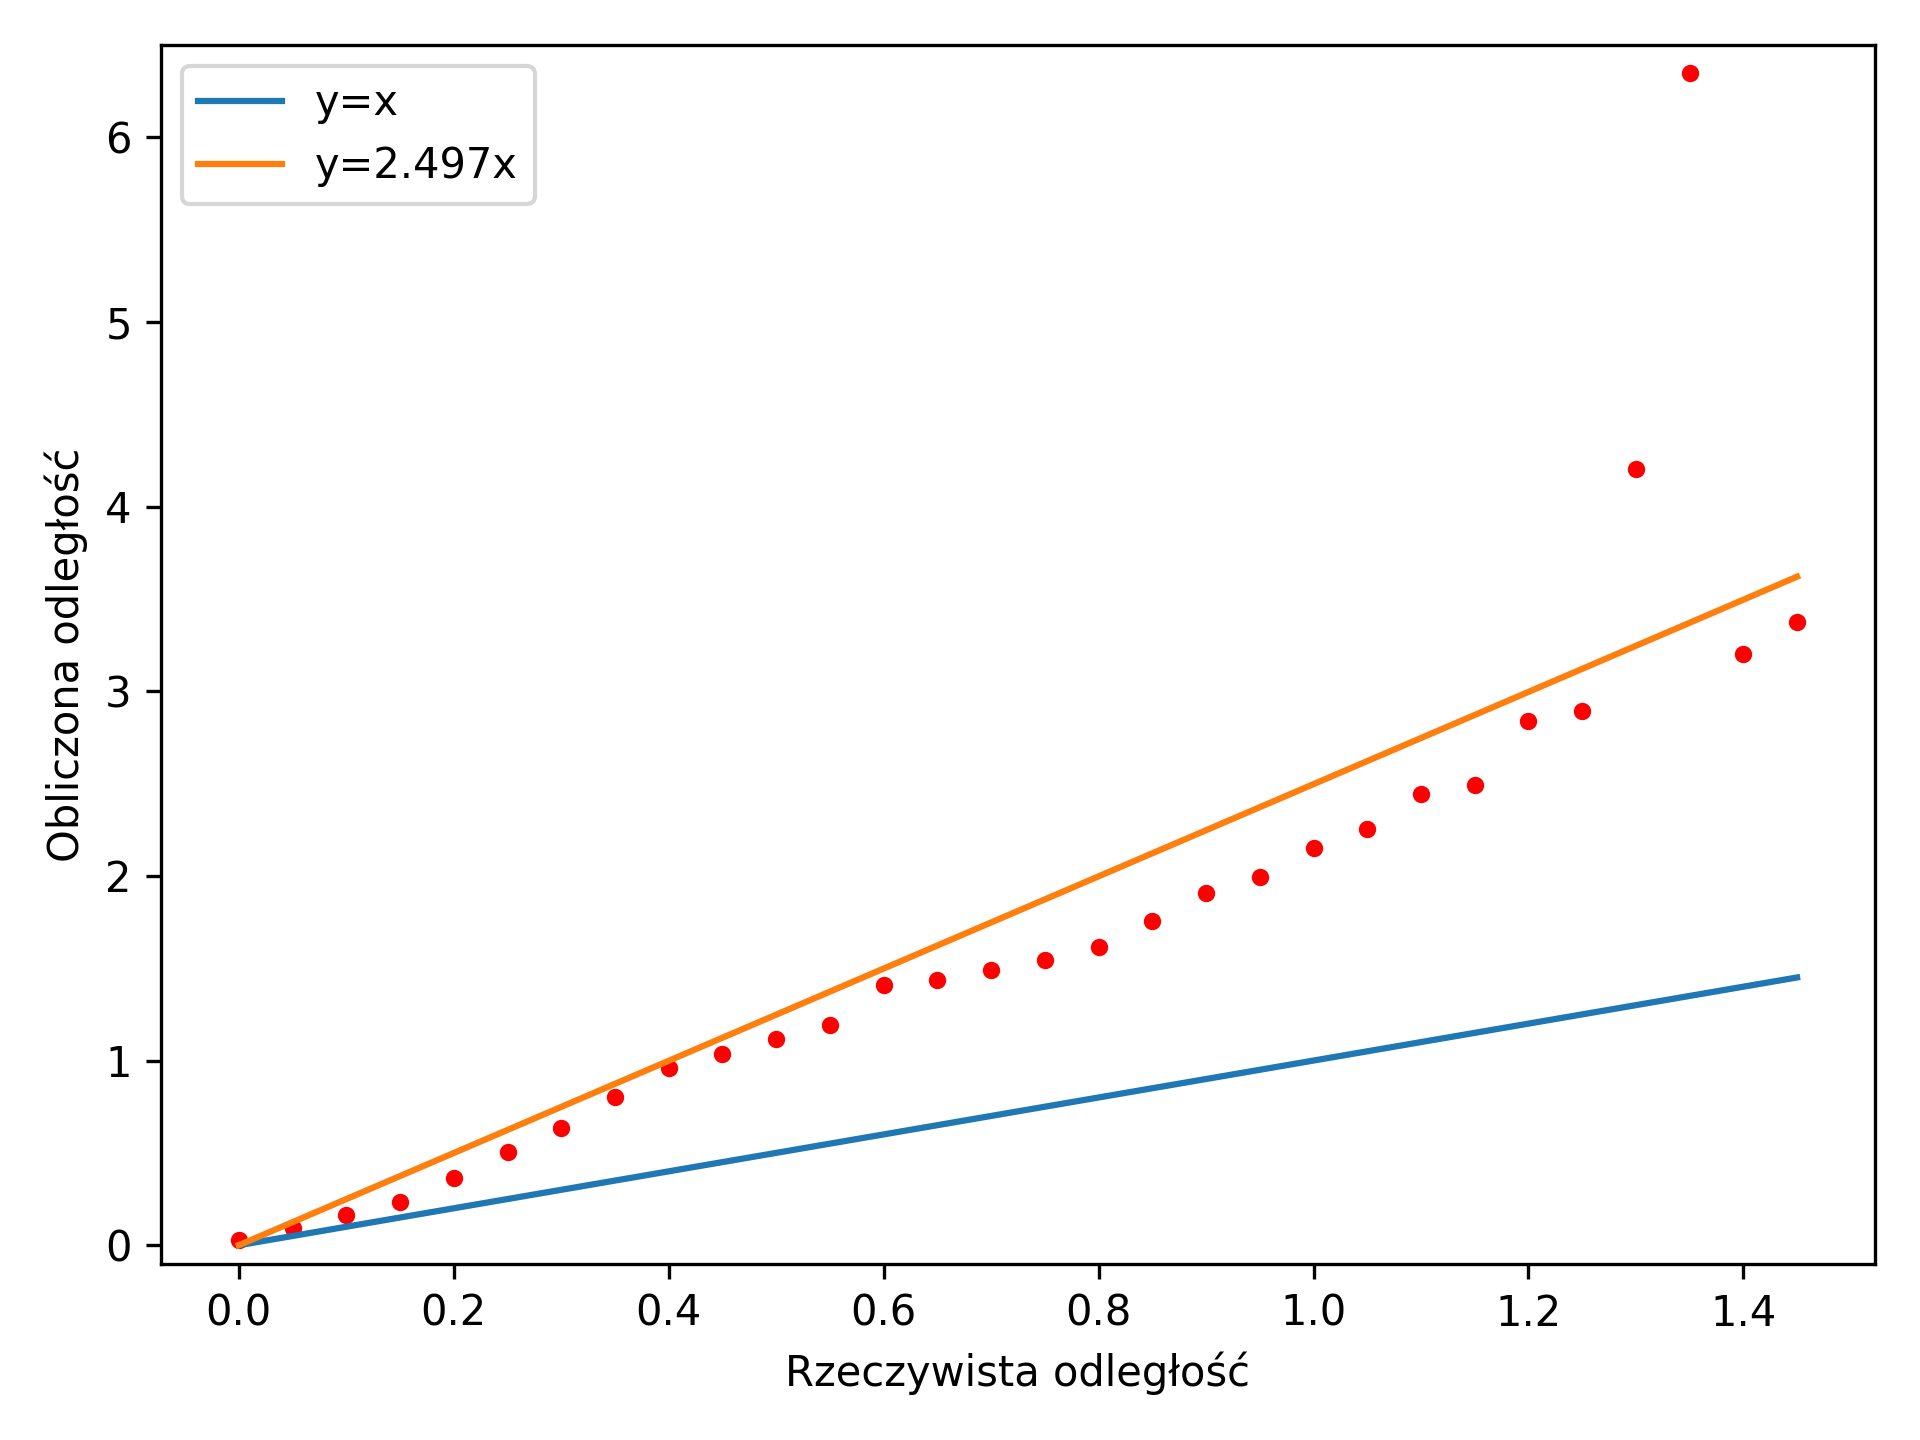
\includegraphics[width=\textwidth]{pics/mic_sync_dist/dists_close_long_1_mean.png}
        \caption{pomiar 2.}
        \label{pic:slope_test_mean_1}
    \end{subfigure}
\end{figure}
\begin{figure}[H]
    \ContinuedFloat\centering
    \begin{subfigure}{0.5\textwidth}
        \centering
        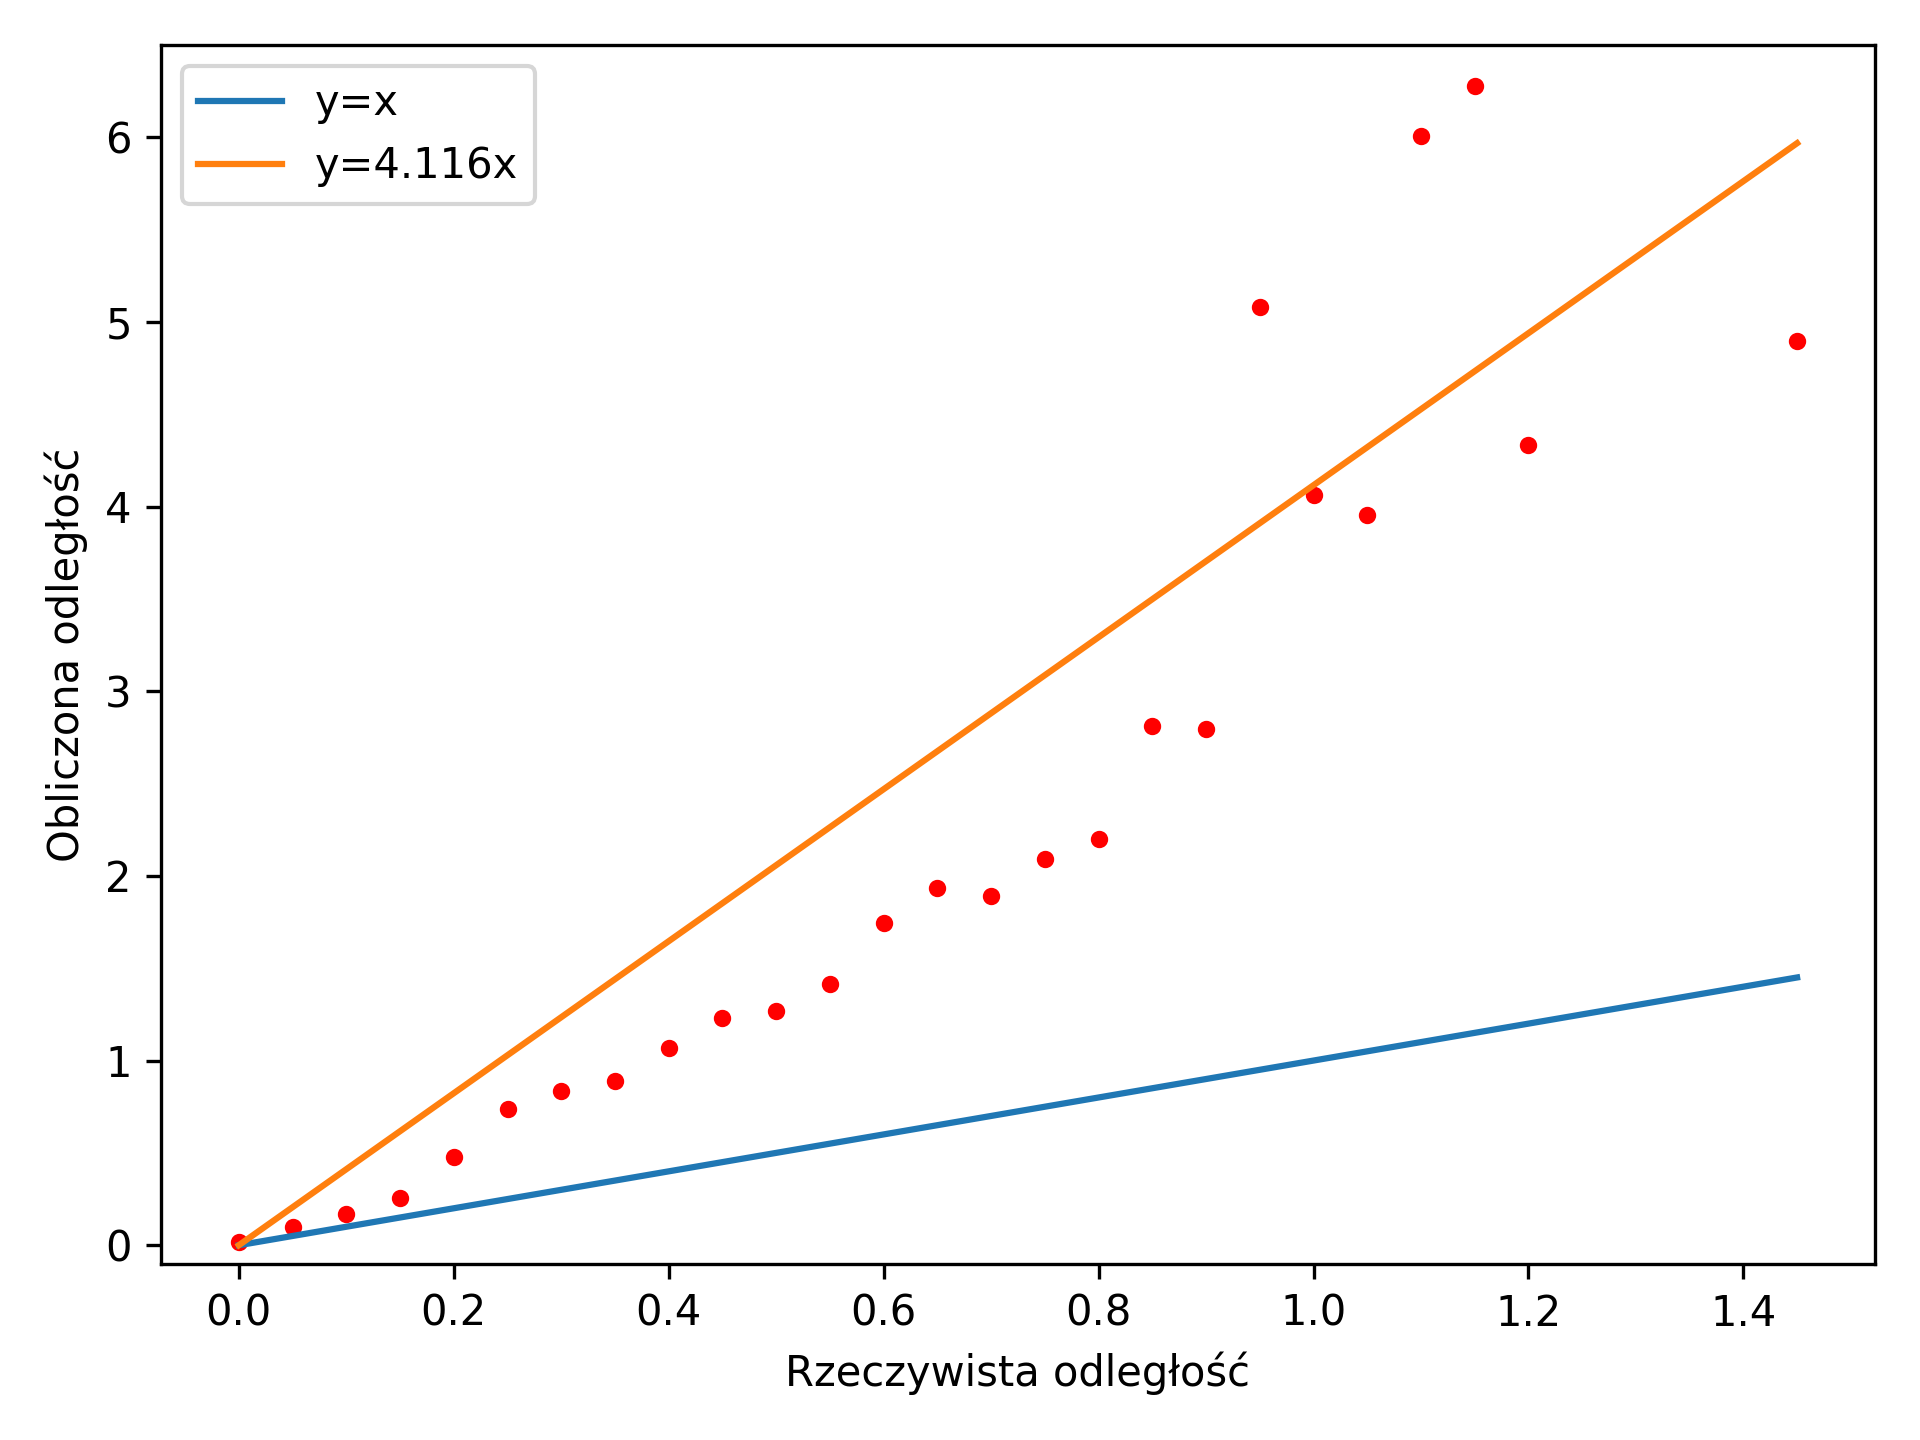
\includegraphics[width=\textwidth]{pics/mic_sync_dist/dists_close_long_2_mean.png}
        \caption{pomiar 3.}
        \label{pic:slope_test_mean_2}
    \end{subfigure}%
    \begin{subfigure}{0.5\textwidth}
        \centering
        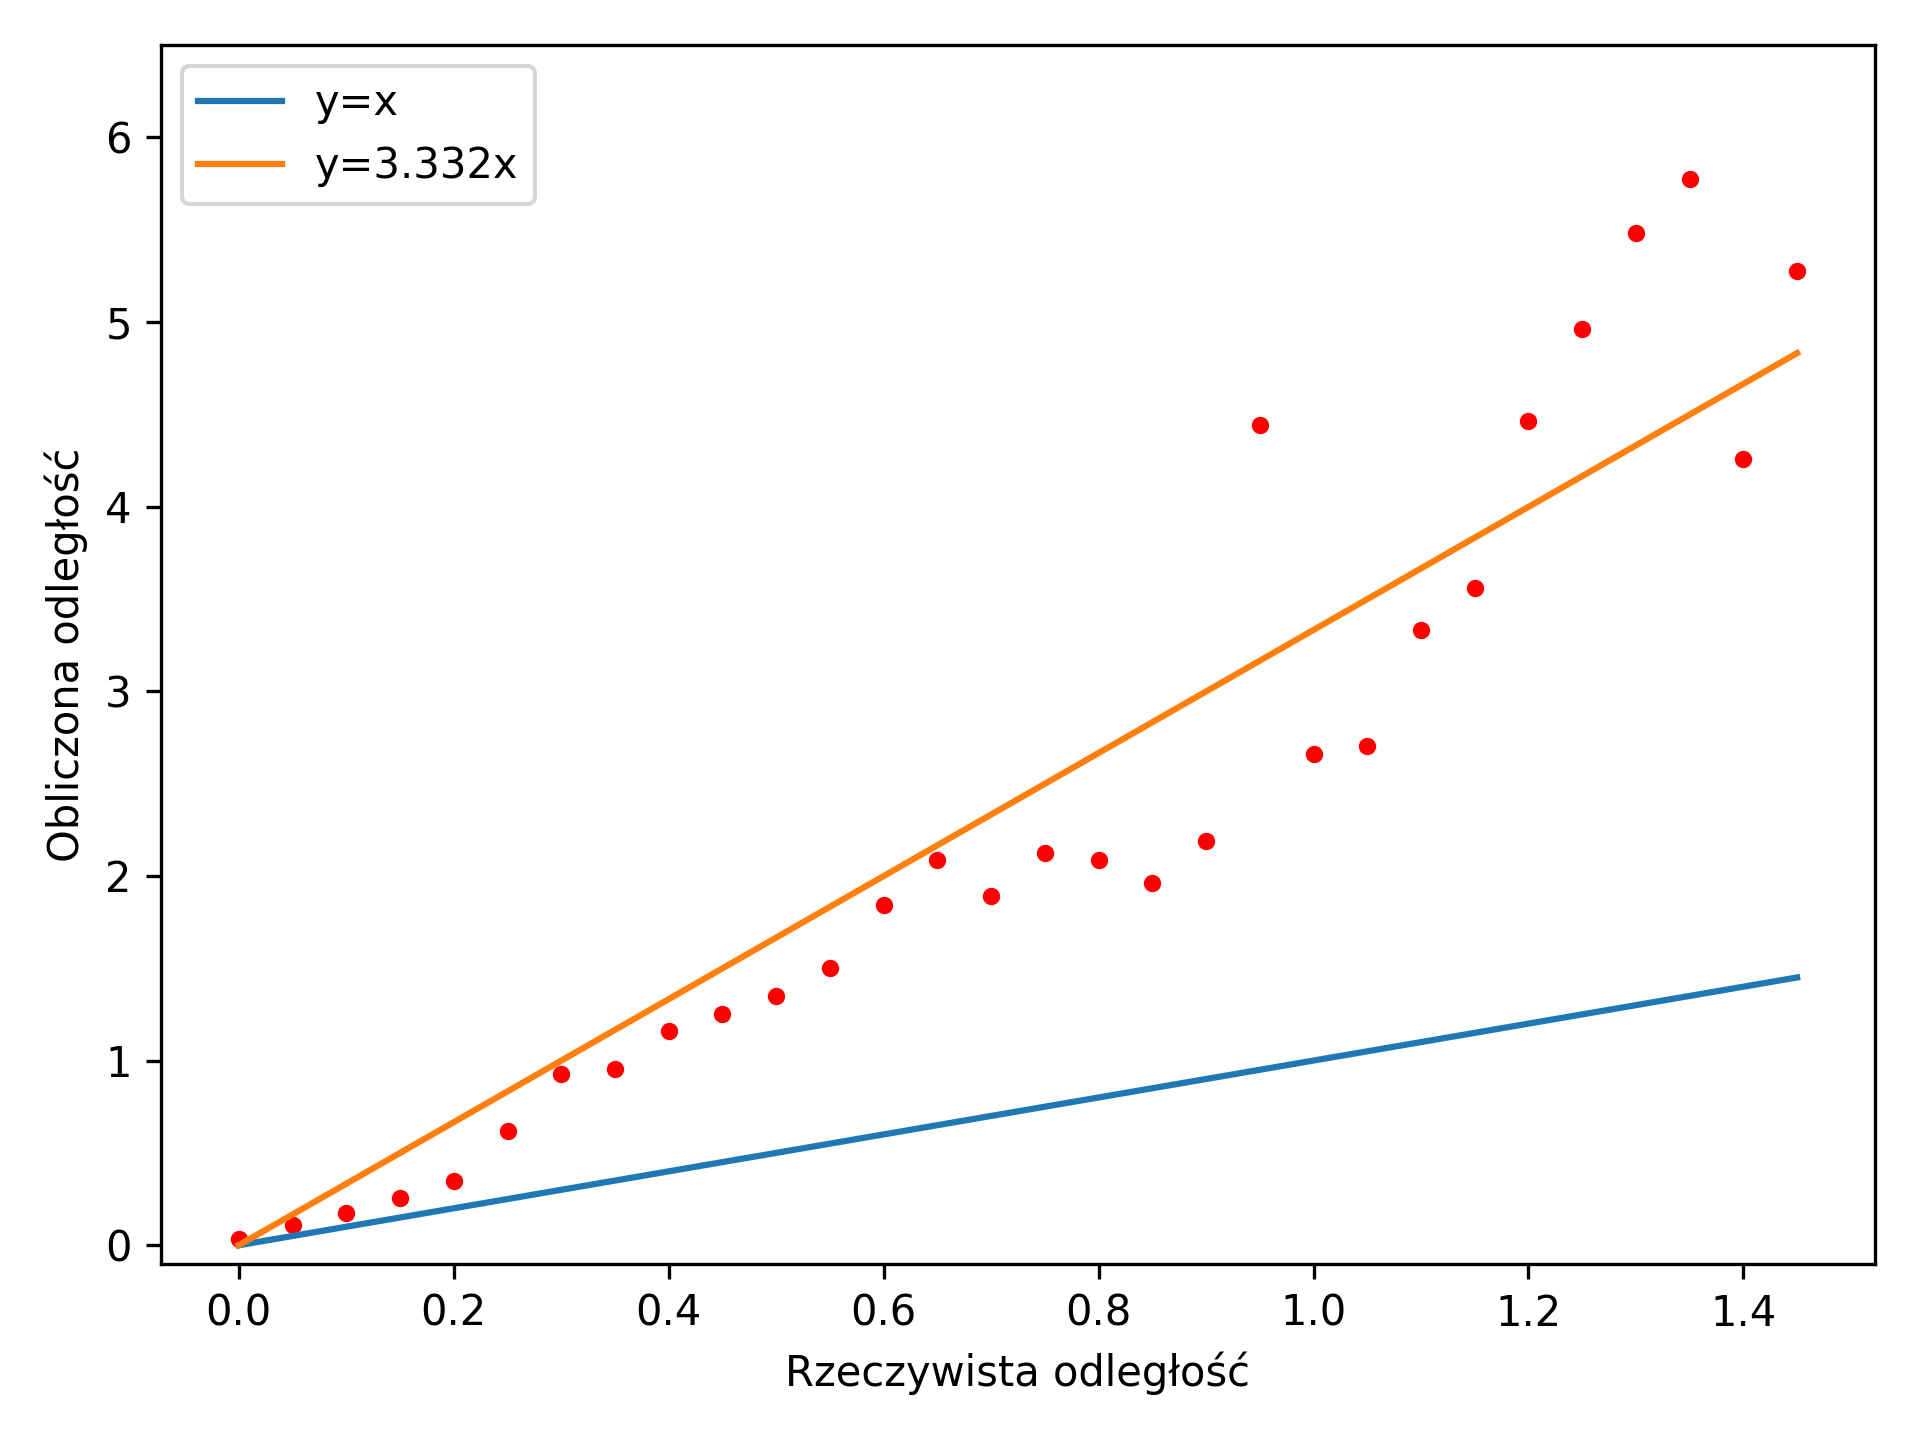
\includegraphics[width=\textwidth]{pics/mic_sync_dist/dists_close_long_3_mean.png}
        \caption{pomiar 4.}
        \label{pic:slope_test_mean_3}
    \end{subfigure}
    \caption{Średnie obliczonych odległości}
    \label{fig:slope_test_mean}
\end{figure}

Na wykresach można zauważyć trendy związane ze zmniejszającą się czułością wzmacniacza mikrofonu:

\begin{itemize}
    \item zmniejszanie się odległości punktu, w którym czułość jest zbyt mała by niezawodnie wyrywać nadawane sygnały,
    \item współczynnik prostej aproksymującej skalowane odległości rośnie.
\end{itemize}

Podobne efekty zaobserwowano, kiedy brzęczyk nie był kierowany bezpośrednio w kierunku odbiornika.

\section{Ocena działania systemu}

W celu oceny działania tak skonstruowanego systemu multilateracyjnego przeprowadzono szereg eksperymentów testujących jego działanie   w zaproponowanych scenariuszach. Bazując na uprzednich obserwacjach, rozszerzono program serwera obliczeniowego tak, aby bezpośrednio przed multilateracją przeprowadzone były synchronizacja czasu oraz korekcja odległości. Zasada działania obu typów węzłów pozostała niezmieniona.

\subsection{Wyniki}

Wyniki eksperymentów przedstawiono na  poniższych wykresach. Mniejsze punkty o wyblakłym kolorze reprezentują badane punkty, w których umieszczony był węzeł nadawczy, natomiast większe, o nasyconym kolorze to odpowiadające im punkty będące uśrednionym wynikiem 25 powtórzeń polecenia lokalizacji w systemie. Wykresy należące do tej samej grupy zachowują skalę w celu łatwiejszego porównania. Dodatkowo, dla przypadku jednowymiarowego, dołączono wybrane wykresy zawierające osobne pomiary każdego z punktów, które składały się na wynik uśredniony.

\subsubsection{Eksperymeny jednowymiarowe}\label{sec:1d}

Ewaluację rozpoczęto, tak jak podczas eksperymentu zerowego, od przypadku jednowymiarowego, aby sprawdzić, czy dokładność i stabilność pomiarów w systemie została poprawiona. Tak samo jak pierwotnie nadajnik umiejscowiono w punkcie $(0)$, natomiast dwa odbiorniki w punktach odpowiednio $(-0,5)$ i $(0,5)$, wszystkie węzły były stacjonarne. Nadajnik co $0,5$ $s$ nadawał sygnał o długości $10$ $ms$, a serwer co $0,5$ $s$ zwracał wynik zagadnienia multilateracji na podstawie ostatnio otrzymanych danych. Następnie zbadano dokładność aproksymacji dla punktów ze zbioru $\{(-0,5; -0,25; 0,25; 0,5)\}$, jak również powtórzono wszystkie pomiary z użyciem dwóch dodatkowych węzłów umiejscowionych w punktach $(-0,25)$ i $(0,25)$. Wyniki przedstawiono na wykresach~\ref{fig:1d_mult_separate} oraz~\ref{fig:1d_mult}.

\begin{figure}[H]
    \centering
    \begin{subfigure}{\textwidth}
        \centering
        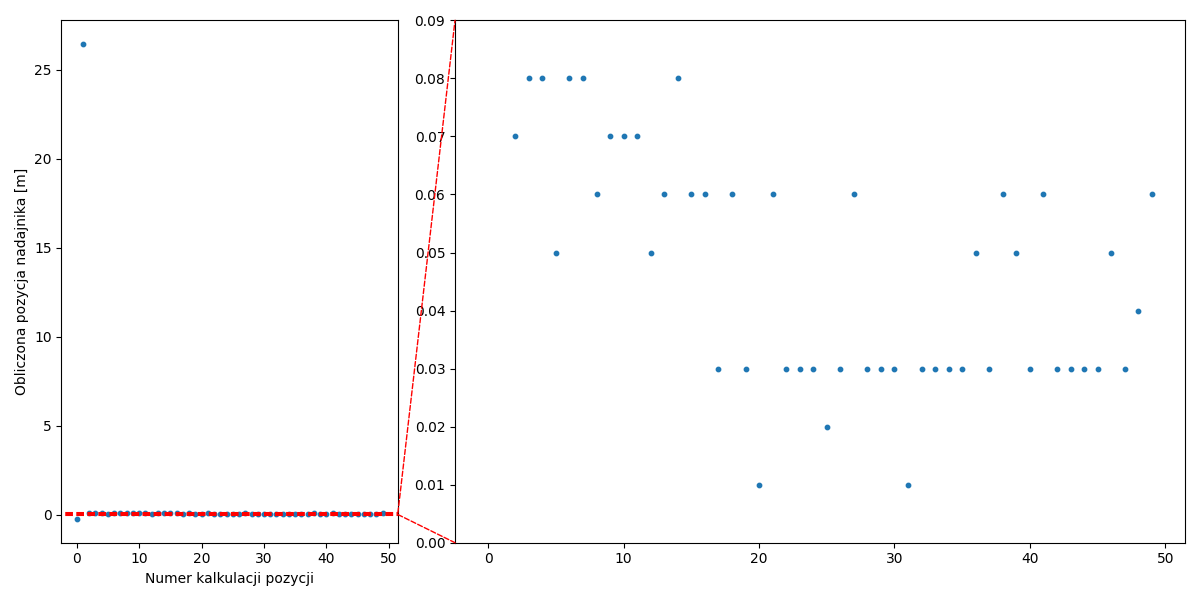
\includegraphics[width=\linewidth]{pics/mult_lat_1d/position_[0]_2.png}
        \caption{Punkt w pozycji (0), 2 mikrofony}
        \label{pic:1d_mult_[0]_2}
    \end{subfigure}
\end{figure}
\begin{figure}[H]
    \ContinuedFloat\centering
    \begin{subfigure}{\textwidth}
        \centering
        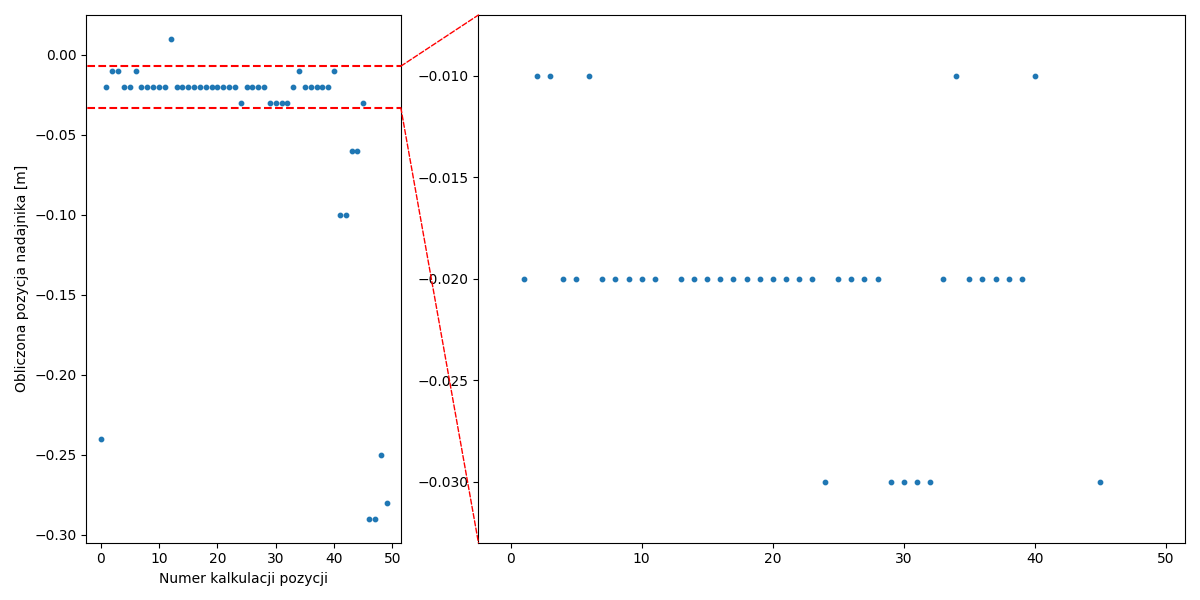
\includegraphics[width=\linewidth]{pics/mult_lat_1d/position_[0]_4.png}
        \caption{Punkt w pozycji (0), 4 mikrofony}
        \label{pic:1d_mult_[0]_4}
    \end{subfigure}
\end{figure}
\begin{figure}[H]
    \ContinuedFloat\centering
    \begin{subfigure}{\textwidth}
        \centering
        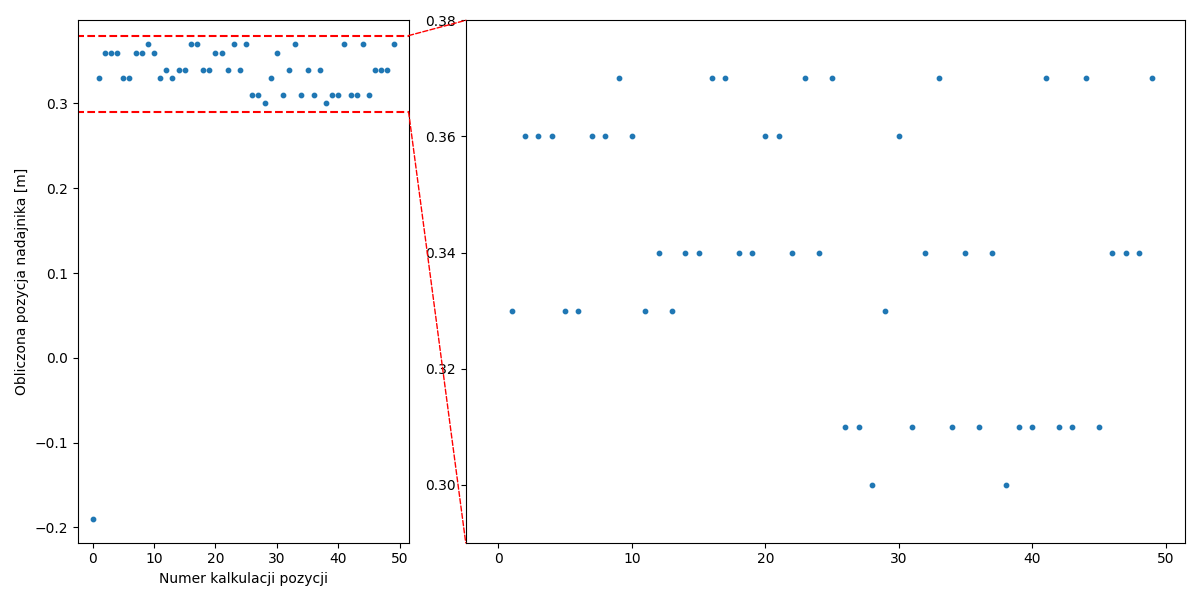
\includegraphics[width=\linewidth]{pics/mult_lat_1d/position_[0.25]_2.png}
        \caption{Punkt w pozycji (0,25), 2 mikrofony}
        \label{pic:1d_mult_[0.25]_2}
    \end{subfigure}
\end{figure}
\begin{figure}[H]
    \ContinuedFloat\centering
    \begin{subfigure}{\textwidth}
        \centering
        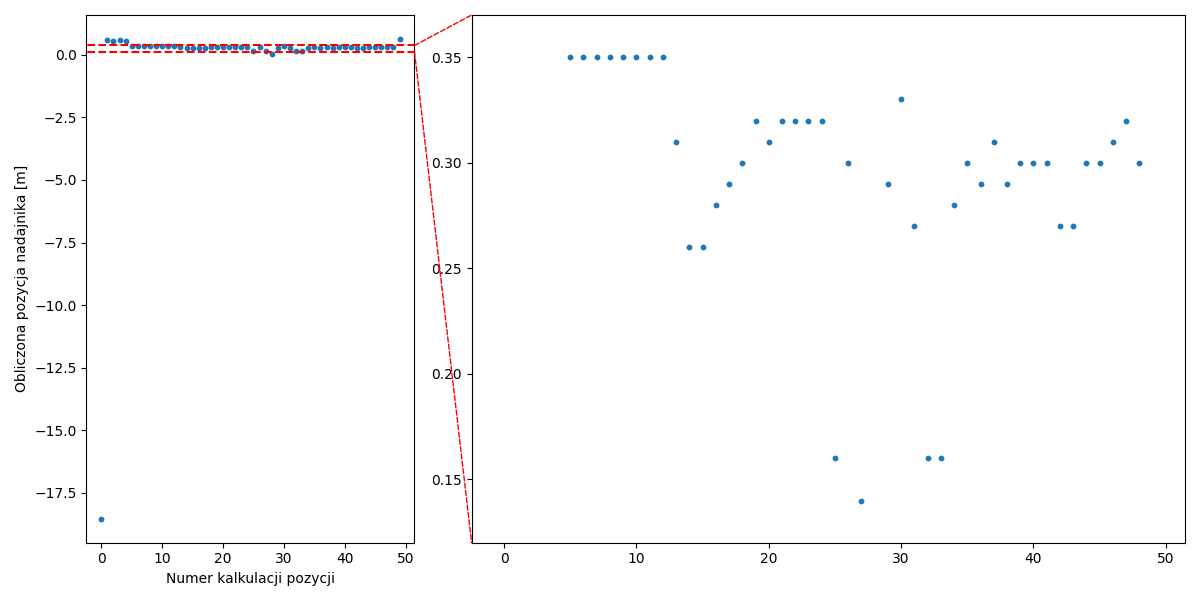
\includegraphics[width=\linewidth]{pics/mult_lat_1d/position_[0.25]_4.png}
        \caption{Punkt w pozycji  (0,25), 4 mikrofony}
        \label{pic:1d_mult_[0.25]_4}
    \end{subfigure}
\end{figure}
\begin{figure}[H]
    \ContinuedFloat\centering
    \begin{subfigure}{\textwidth}
        \centering
        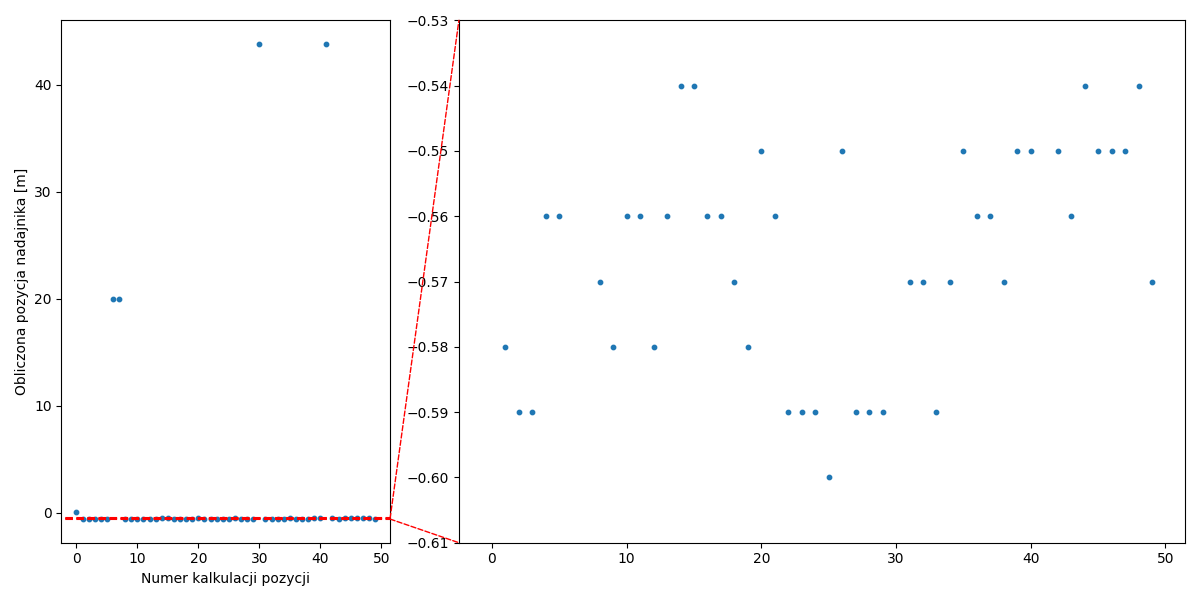
\includegraphics[width=\linewidth]{pics/mult_lat_1d/position_[-0.5]_2.png}
        \caption{Punkt w pozycji  (-0,5), 2 mikrofony}
        \label{pic:1d_mult_[-0.5]_2}
    \end{subfigure}
\end{figure}
\begin{figure}[H]
    \ContinuedFloat\centering
    \begin{subfigure}{\textwidth}
        \centering
        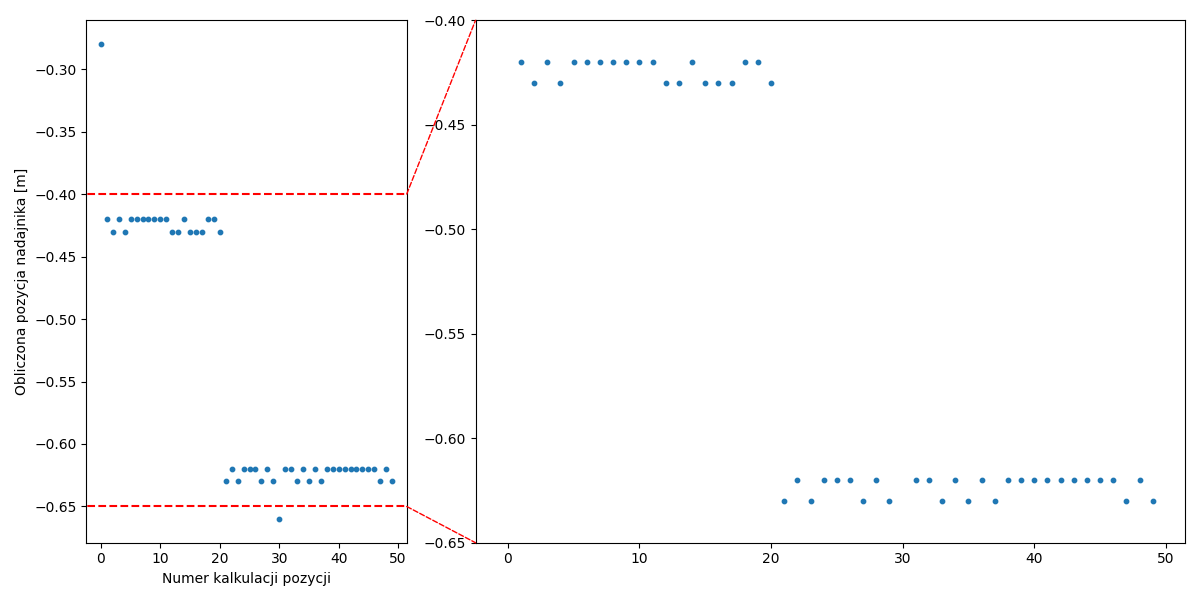
\includegraphics[width=\linewidth]{pics/mult_lat_1d/position_[-0.5]_4.png}
        \caption{Punkt w pozycji  (-0,5), 4 mikrofony}
        \label{pic:1d_mult_[-0.5]_4}
    \end{subfigure}
    \caption{Wykres obliczonej pozycji odbiornika w zależności od czasu}
    \label{fig:1d_mult_separate}
\end{figure}

\begin{figure}[H]
    \centering
    \begin{subfigure}{.5\textwidth}
        \centering
        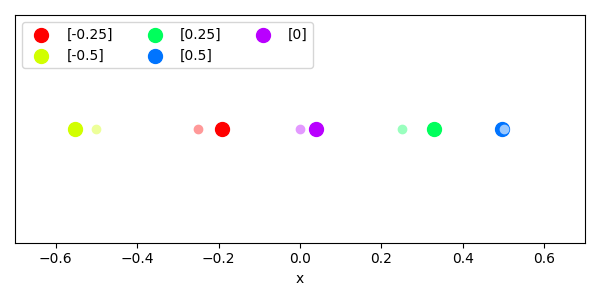
\includegraphics[width=\linewidth]{pics/mult_lat_1d/positions_2_mean.png}
        \caption{2 mikrofony}
        \label{pic:1d_2_mult}
    \end{subfigure}%
    \begin{subfigure}{.5\textwidth}
        \centering
        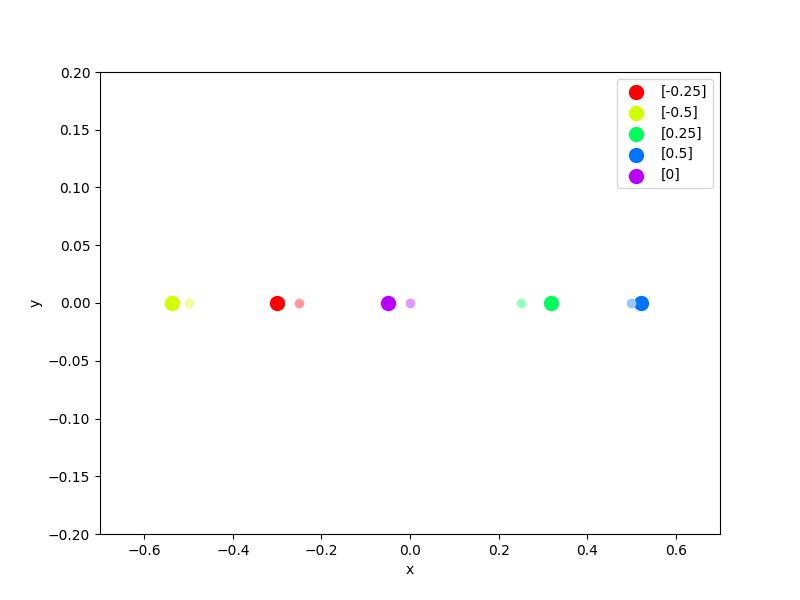
\includegraphics[width=\linewidth]{pics/mult_lat_1d/positions_4_mean.png}
        \caption{4 mikrofony}
        \label{pic:1d_4_mult}
    \end{subfigure}
    \caption[Wyniki eksperymentu dla wersji 1D]{Średnie obliczonych pozycji, wariant 1D. Małe, blade kropki to kolejne punkty testowe, w których umieszczano nadajnik, a duże kropki to średnie wyników zwracanych przez system multilateracyjny. Każdy kolor to inny punkt testowy o koordynatach podanych w legendzie.}
    \label{fig:1d_mult}
\end{figure}

\subsubsection{Eksperymenty dwuwymiarowe}

Następnie sprawdzono system w wariancie dwuwymiarowym. Aby zachować podobną maksymalną odległość pomiędzy odbiornikami, zdecydowano się na umiejscowienie czterech węzłów na wierzchołkach kwadratu o boku $0,6$ symetrycznie względem puntu $(0;0)$, a więc na punktach o współrzędnych $(\pm0,3; \pm0,3)$. Zbadano dokładność lokalizacji w trzech zestawach punktów:

\begin{itemize}
    \item $\{(0;0), (0,3;0,3), (-0,3;0,3), (-0,3;-0,3), (0,3;-0,3)\}$
    \item $\{(0;0), (0;0,3), (0;-0,3), (-0,3;0), (0,3;0)\}$
    \item $\{(0;0), (0,15;0,15), (-0,15;0,15), (-0,15;-0,15), (0,15;-0,15)\}$
\end{itemize}
Wyniki przedstawiono na wykresach~\ref{fig:2d_mult}.

\begin{figure}[H]
    \centering
    \begin{subfigure}{.5\textwidth}
        \centering
        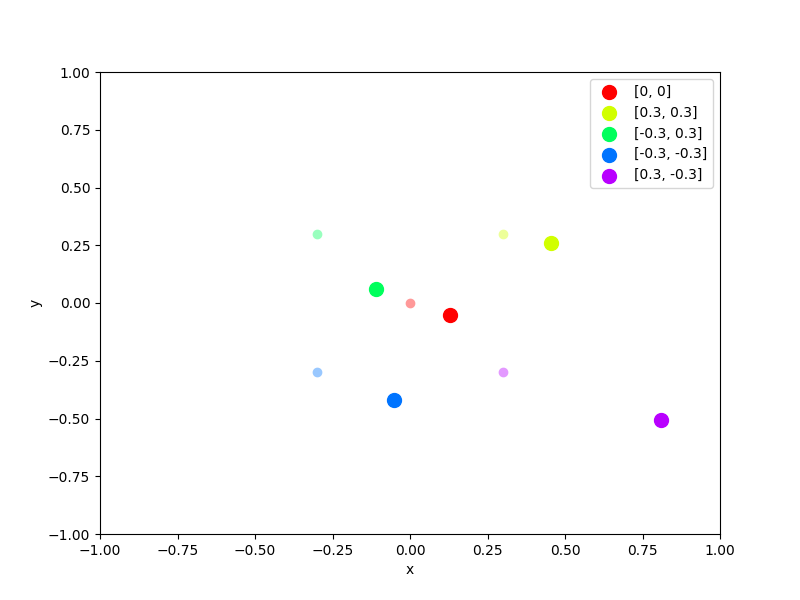
\includegraphics[width=\linewidth]{pics/mult_lat_2d/positions_1_mean.png}
        \caption{zestaw punktów 1.}
        \label{pic:2d_1_mult}
    \end{subfigure}%
    \begin{subfigure}{.5\textwidth}
        \centering
        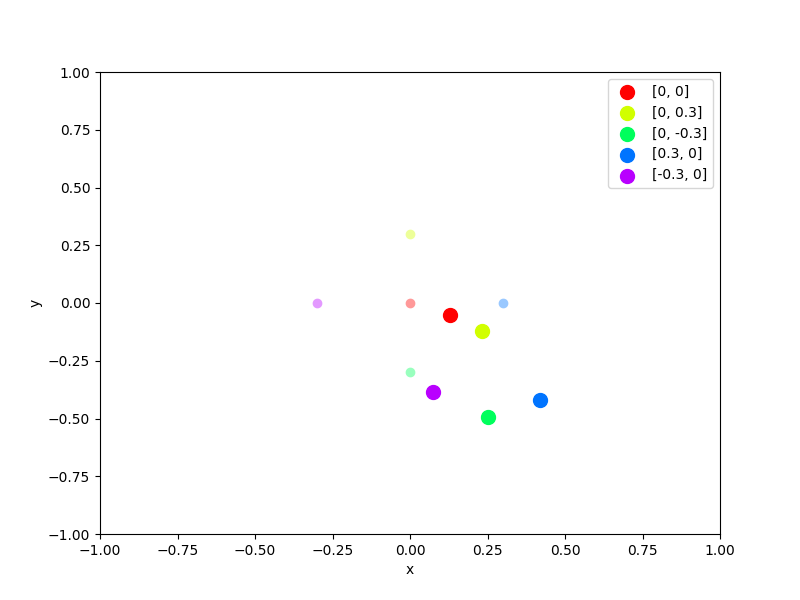
\includegraphics[width=\linewidth]{pics/mult_lat_2d/positions_2_mean.png}
        \caption{zestaw punktów 2.}
        \label{pic:2d_2_mult}
    \end{subfigure}
\end{figure}
\begin{figure}[H]
    \ContinuedFloat\centering
    \begin{subfigure}{.5\textwidth}
        \centering
        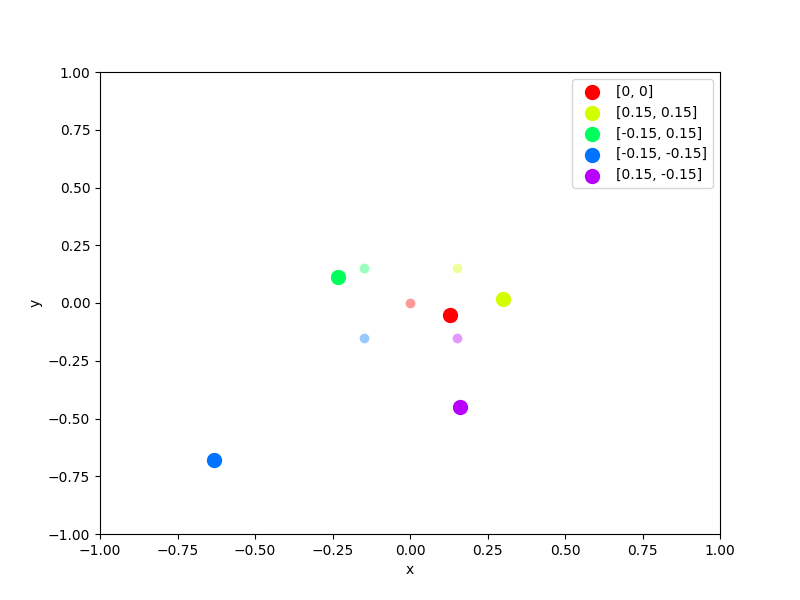
\includegraphics[width=\linewidth]{pics/mult_lat_2d/positions_3_mean.png}
        \caption{zestaw punktów 3.}
        \label{pic:2d_3_mult}
    \end{subfigure}
    \caption[Wyniki eksperymentu dla wersji 2D]{Średnie obliczonych pozycji, wariant 2D. Małe, blade kropki to kolejne punkty testowe, w których umieszczano nadajnik, a duże kropki to średnie wyników zwracanych przez system multilateracyjny. Każdy kolor to inny punkt testowy o koordynatach podanych w legendzie.}
    \label{fig:2d_mult}
\end{figure}

Następnie w celu ewaluacji wpływu charakterystyki otoczenia na działanie systemu przeprowadzono trzy następujące bezpośrednio po sobie eksperymenty zachowując ustaloną na początku synchronizację zegarów i stałe korekcji odległości. Sprawdzono dokładność estymacji tego samego zbioru punktów wyjściowo oraz po rotacji całego układu o $45^{\circ}$ i $90^{\circ}$ zgodnie z ruchem wskazówek zegara. Wyniki przedstawiono na wykresach~\ref{fig:2d_angle_mult}. 

\begin{figure}[H]
    \centering
    \begin{subfigure}{.5\textwidth}
        \centering
        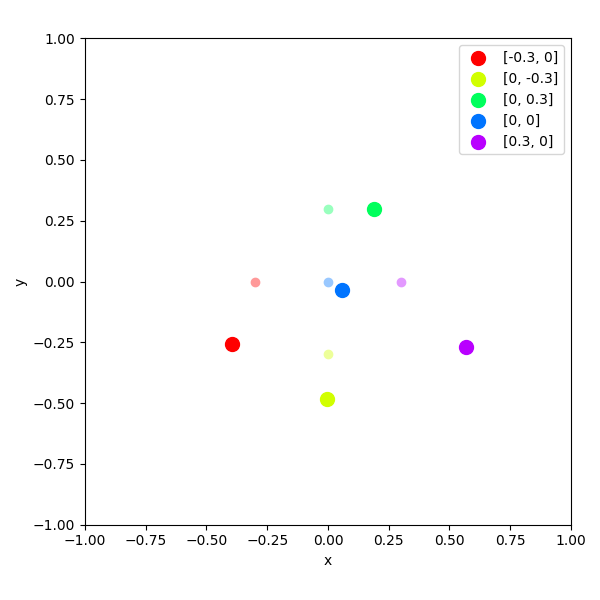
\includegraphics[width=\linewidth]{pics/mult_lat_2d_angle/positions_0_mean.png}
        \caption{rotacja $0^{\circ}$}
        \label{pic:2d_0_angle_mult}
    \end{subfigure}%
    \begin{subfigure}{.5\textwidth}
        \centering
        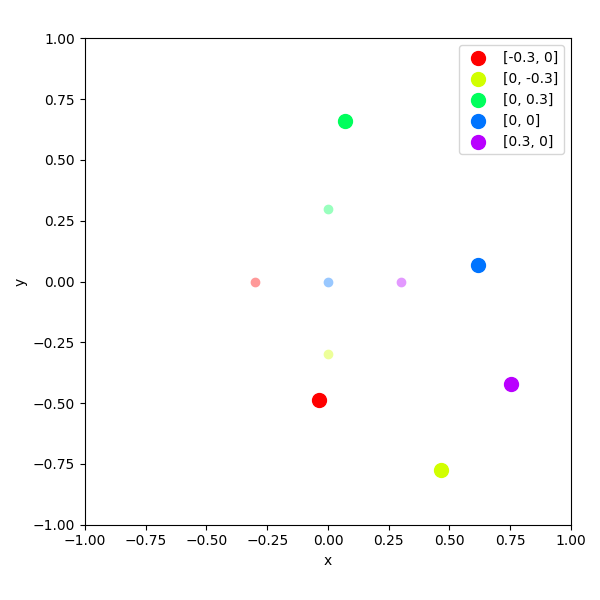
\includegraphics[width=\linewidth]{pics/mult_lat_2d_angle/positions_45_mean.png}
        \caption{rotacja $45^{\circ}$}
        \label{pic:2d_45_angle_mult}
    \end{subfigure}
\end{figure}
\begin{figure}[H]
    \ContinuedFloat\centering
    \begin{subfigure}{.5\textwidth}
        \centering
        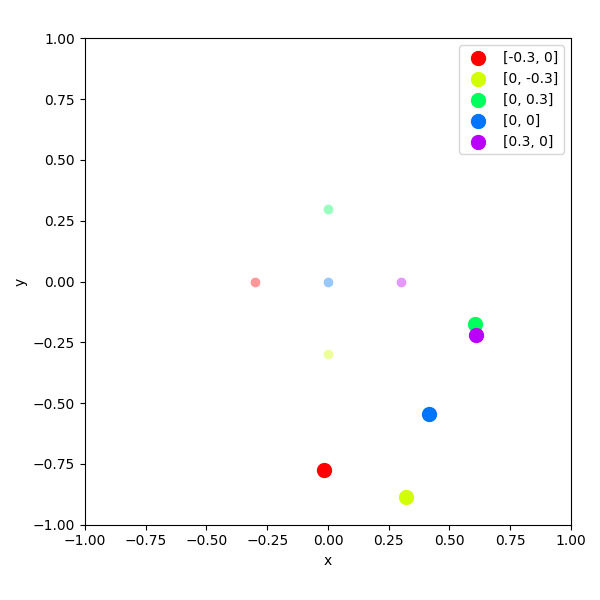
\includegraphics[width=\linewidth]{pics/mult_lat_2d_angle/positions_90_mean.png}
        \caption{rotacja $90^{\circ}$}
        \label{pic:2d_90_angle_mult}
    \end{subfigure}
    \caption[Wyniki eksperymentu dla wersji 2D z rotacją]{Średnie obliczonych pozycji, wariant 2D z rotacją. Małe, blade kropki to kolejne punkty testowe, w których umieszczano nadajnik, a duże kropki to średnie wyników zwracanych przez system multilateracyjny. Każdy kolor to inny punkt testowy o koordynatach podanych w legendzie.}
    \label{fig:2d_angle_mult}
\end{figure}

Ostatecznie sprawdzono zachowanie systemu wraz ze zmianą liczby węzłów odbiorczych od minimalnej liczby trzech aż do ośmiu. Węzły umiejscowiono na punktach ze zbioru $\{(0,3;0,3), (-0,3;0,3), (-0,3;-0,3), (0,3;-0,3), (0; 0,425), (-0,425; 0), (0; -0,425), (0,425; 0)\}$ oraz dodawano je zgodnie z tą kolejnością. Wyniki przedstawiono na wykresach~\ref{fig:2d_num_mult}. 

\begin{figure}[H]
    \centering
    \begin{subfigure}{.5\textwidth}
        \centering
        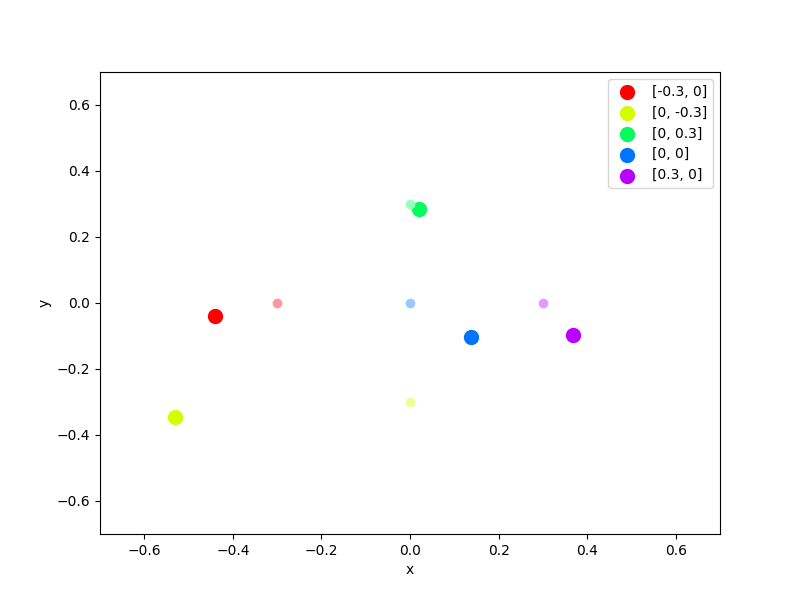
\includegraphics[width=\linewidth]{pics/mult_lat_2d_num/positions_3_mean.png}
        \caption{3 mikrofony}
        \label{pic:2d_3_num_mult}
    \end{subfigure}%
    \begin{subfigure}{.5\textwidth}
        \centering
        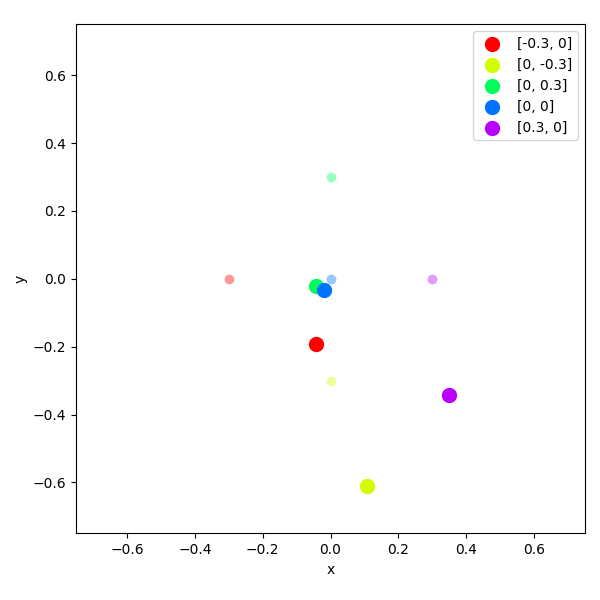
\includegraphics[width=\linewidth]{pics/mult_lat_2d_num/positions_4_mean.png}
        \caption{4 mikrofony}
        \label{pic:2d_4_num_mult}
    \end{subfigure}
\end{figure}
\begin{figure}[H]
    \ContinuedFloat\centering
    \begin{subfigure}{.5\textwidth}
        \centering
        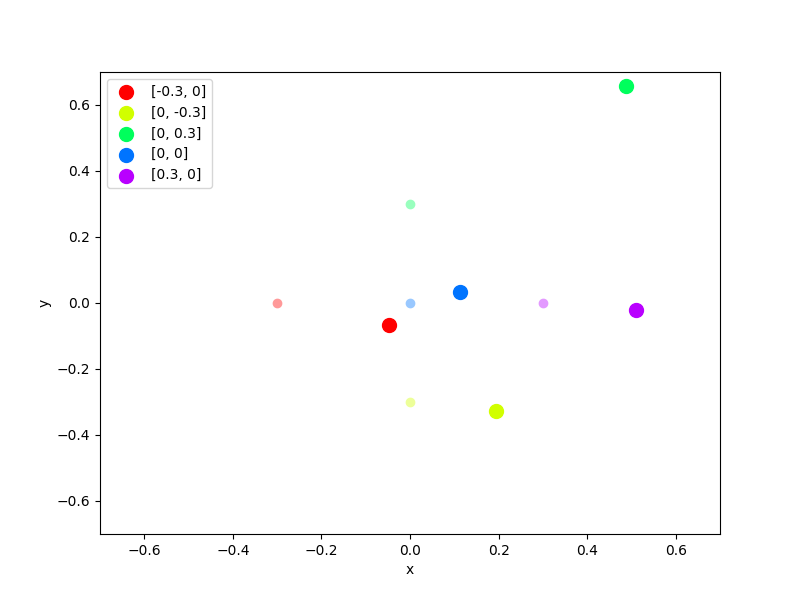
\includegraphics[width=\linewidth]{pics/mult_lat_2d_num/positions_5_mean.png}
        \caption{5 mikrofonów}
        \label{pic:2d_5_num_mult}
    \end{subfigure}%
    \begin{subfigure}{.5\textwidth}
        \centering
        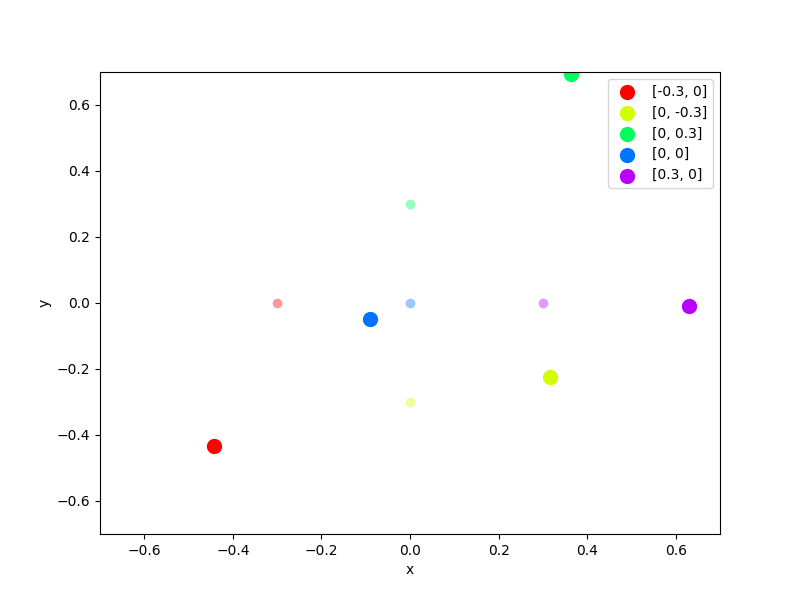
\includegraphics[width=\linewidth]{pics/mult_lat_2d_num/positions_6_mean.png}
        \caption{6 mikrofonów}
        \label{pic:2d_6_num_mult}
    \end{subfigure}
\end{figure}
\begin{figure}[H]
    \ContinuedFloat\centering
    \begin{subfigure}{.5\textwidth}
        \centering
        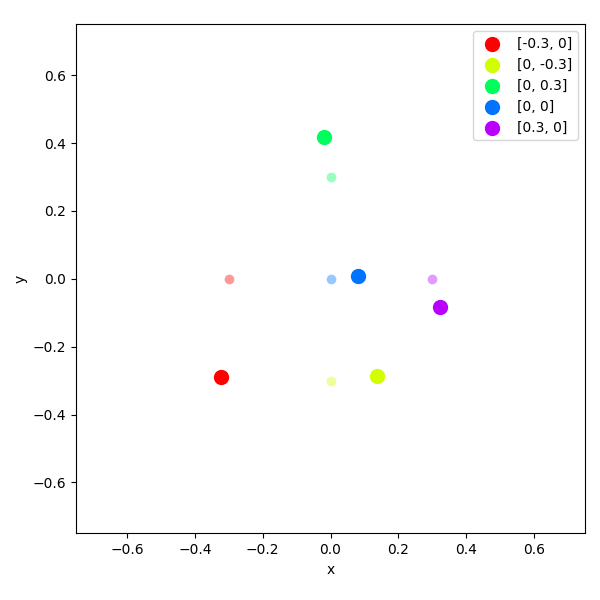
\includegraphics[width=\linewidth]{pics/mult_lat_2d_num/positions_7_mean.png}
        \caption{7 mikrofonów}
        \label{pic:2d_7_num_mult}
    \end{subfigure}%
    \begin{subfigure}{.5\textwidth}
        \centering
        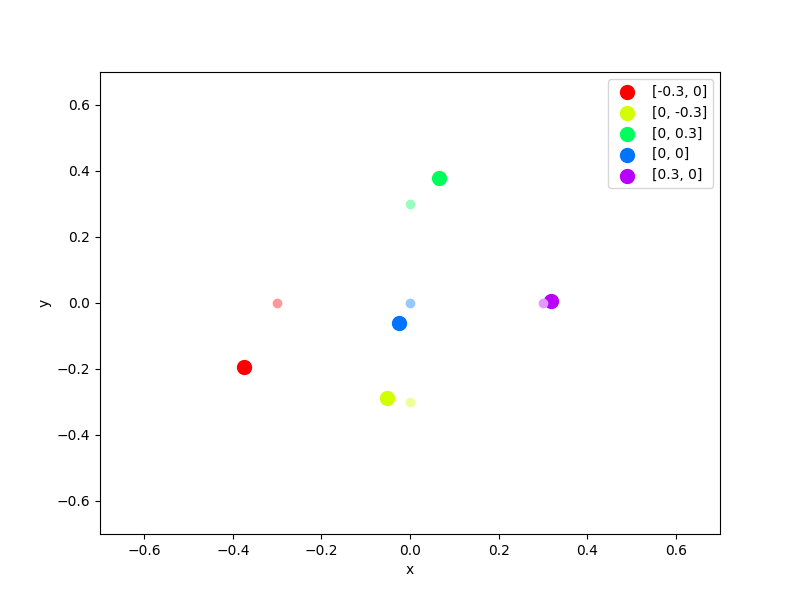
\includegraphics[width=\linewidth]{pics/mult_lat_2d_num/positions_8_mean.png}
        \caption{8 mikrofonów}
        \label{pic:2d_8_num_mult}
    \end{subfigure}
    \caption[Wyniki eksperymentu dla wersji 2D ze zmienną liczbą mikrofonów]{Średnie obliczonych pozycji, wariant 2D ze zmienną liczbą mikrofonów. Małe, blade kropki to kolejne punkty testowe, w których umieszczano nadajnik, a duże kropki to średnie wyników zwracanych przez system multilateracyjny. Każdy kolor to inny punkt testowy o koordynatach podanych w legendzie.}
    \label{fig:2d_num_mult}
\end{figure}

\section{Interpretacja i wnioski}

Rozpoczynając od porównania wyników eksperymentu zerowego z rodziału~\ref{chap:experiment_zero} z wynikami przypadku jednowymiarowego (sekcja \ref{sec:1d}), można od razu zauważyć poprawę zarówno dokładności jak i stabilności pomiarów. W pierwszej kolejności zwróćmy uwagę na znaczne zmniejszenie przesunięcia obliczanych lokalizacji nadajnika względem jego prawdziwego położenia, które wynika z zastosowania synchronizacji sprzętowej, opisanej w sekcji~\ref{sec:mic_sync}, biorącej pod uwagę wszelkie opóźnienia pomijane w przypadku synchronizacji sprzętowej (sekcja \ref{sec:prog_sync}). Ponadto dokładność wyników multilateracji nie ulega gwałtownemu spadkowi wraz z upływem czasu (wyjątkiem w poprawionych eksperymentach jest przypadek przedstawiony na wykresie~\ref{pic:1d_mult_[-0.5]_4}, w którym zauważalna jest nagła zmiana średniej lokalizowanych punktów, czego przyczyną mogło być prawdopodobnie zmiana warunków otoczenia eksperymentu). Ostateczne wyniki multilateracji jednowymiarowej przedstawione na rysunku~\ref{fig:1d_mult} wskazują na zadowalającą (w zależności od zastosowań) dokładność pomiaru położenia nadajnika.

Przypadek jednowymiarowy jest jednak na tyle zdegenerowany, że do jego rozwiązania nie jest konieczne użycie metod multilateracyjnych, dlatego decydującym o użyteczności systemu było testowanie w wariancie dwuwymiarowym. Wyniki pierwszych testów (\ref{fig:2d_mult}) nie były obiecujące {-} układ punktów względem siebie był w przybliżeniu zachowany, jednak punkty zwracane przez system znajdują się czasami w znacznej odległości od ich rzeczywistych położeń. Kolejne dwie serie testów, przeprowadzone w celu sprawdzenia jakie aspekty wpływają pozytywnie, a jakie negatywnie na dokładność lokalizacji wykazały dwie zależności:
\begin{itemize}
    \item podatność systemu na zmiany charakterystyki sonicznej otocznia (\ref{fig:2d_angle_mult});
    \item wzrost dokładności lokalizacji wraz ze wzrostem liczby węzłów odbiorczych (\ref{fig:2d_num_mult}).
\end{itemize}
Pierwsza z zależności jest wyraźnie widoczna, ponieważ wraz z obrotem układu węzłów względem otoczenia błąd lokalizacji rośnie, jak również położenie punktów względem siebie ulega zmianie do tego stopnia, że trudno odgadnąć jaki kształt tworzyły w rzeczywistości. Druga zależność nie jest tak wydatna jak poprzednia, ponieważ błąd lokalizacji każdego z punktów nie jest ściśle malejący, czasem większa liczba węzłów nadawczych nie pomaga, a może nawet przeszkadzać (kolejny dodany węzeł mógł mieć niepoprawnie ustawioną czułość wzmacniacza, co znacznie wpłynęłoby na wyniki przy małej liczbie węzłów). Po zwiększeniu liczby do 7 i 8 widać zalety skali w takim systemie {-} nawet jeśli któraś z raportowanych odległości jest obarczona znaczącym błędem, rozwiązanie aproksymacyjne minimalizujące sumę kwadratów błędów będzie bliższe punktowi, na który wskazują odległości podane przez pozostałe węzły.
